% !TeX encoding = UTF-8
% !TeX program = xelatex
% !TeX spellcheck = en_US

\documentclass[master,pdf]{ustcthesis}
% doctor|master|bachelor [academic|professional] [chinese|english] [print|pdf]
% [super|numebers|authoryear]

\title{基于风云四号卫星数据的\\雷暴区域特征提取}
\author{宋刘幸}
\major{信息工程}
\supervisor{王博\ 讲师}
\date{二〇一九年五月} % 注释掉则为今日
% \professionaltype{专业学位类型}
% \secretlevel{秘密}        % 绝密|机密|秘密,注释本行则不保密
% \secretyear{20}           % 保密年限

\entitle{Feature Extraction of Thunderstorm Area Based on FY4A Satellite Data}
\enauthor{Liuxing Song}
\enmajor{Information engineering}
\ensupervisor{Bo Wang}
%\encosupervisor{Prof. Xuesen Qian}
\endate{May , 2019}      % Today if commented
% \enprofessionaltype{Professional degree type}
% \ensecretlevel{Secret}    % Top secret|Highly secret|Secret


% 加载宏包和配置
\usepackage{graphicx}
\usepackage{subfigure}
\graphicspath{{figures/}}
\usepackage{booktabs}
\usepackage{longtable}
\usepackage[ruled,linesnumbered]{algorithm2e}
\usepackage{siunitx}
\usepackage{amsthm}
\usepackage{hyperref}
\usepackage{natbib}

\DeclareRobustCommand\cs[1]{\texttt{\char`\\#1}}
\newcommand\pkg{\textsf}

\renewcommand\vec{\symbf}
\newcommand\mat{\symbf}
\newcommand\ts{\symbfsf}
\newcommand\real{\mathbf{R}}




\begin{document}

% 研究生论文:
%   封面,原创性声明和授权使用声明
%   frontmatter: 摘要,目录,[图、表清单],[符号说明]
%   mainmatter: 正文章节,参考文献
%   appendix: 附录
%   backmatter: 致谢,已发表论文列表
%
% 本科生论文:
%   封面
%   frontmatter: 致谢,目录,摘要
%   mainmatter: 正文章节,参考文献
%   appendix: 附录

\maketitle
%\makestatement
\bibliographystyle{plain}
\frontmatter
% !TeX root = . . /main. tex

\begin{abstract}
  常规的雷暴探测,主要借助自动气象站、闪电定位仪、雷达、探空等技术手段,但是,
  由于雷暴发生的时空尺度较小,常规气象探测手段的短期临近预报能力较弱,
  对雷暴、强风、强降雨等灾害天气的虚报漏报率较高。
  通过对高精度的风云四号卫星数据进行处理,充分挖掘云图中与雷暴区域相关性强的云区信息,
  从图像角度提取雷暴区域云图的相关特征,利用数字图像处理理论,本文提出一种根据纹理特征阈值判断雷暴云的方法,
  从而提高对雷暴天气的监测和预警能力。经测试库测试,本文提出的方法,预警率可达到90$\%$以上。

  \keywords{风云四号;特征提取;雷暴预警}
\end{abstract}

\begin{enabstract}
  \iffalse
  Conventional thunderstorm detection, mainly by means of automatic weather stations, 
  lightning locators, radar, sounding and other technical means.  However, due to the small spatial and temporal scale of thunderstorms, 
  the short-term nowcasting capability of conventional meteorological means is still 
  very low. The false report and false negative rate of disaster weather 
  such as thunderstorms, strong winds and heavy rainfall are still high. This article uses digital image processing theory 
  by processing the high-precision FY4A satellite data. The cloud area feature information with strong correlation 
  with the thunderstorm area in the cloud map is fully tapped. The related features of thunderstorm region cloud map are extracted from the image, 
  and a method for judging thunderstorm cloud based on texture feature threshold is proposed. 
  Improving monitoring and early warning capabilities for thunderstorms. 
  After the test library test, the method proposed in this paper can reach more than 90$\%$. 
\fi

  Conventional thunderstorm detection, mainly by automatic weather stations, lightning locators, radar, sounding and other technical means. However, due to the small spatial and temporal scale of thunderstorms, the short-term nowcasting capability of conventional meteorological means is still 
  weak. The rate of false positives and false negatives of disaster weather 
  such as thunderstorms, strong winds and heavy rainfall are still high. With 
  processing the high-precision FY4A satellite data, digging thunderstorm-correlative cloud area information and extracting 
  image features of the cloud map of thunderstorm area, this paper, combined with digital image processing theory, 
  comes up with a method for judging thunderstorm cloud based on texture feature threshold to improve monitoring and early 
  warning capabilities for thunderstorms. Testing in the test library, the method proposed in this paper can reach an accuracy of more than 90$\%$. 
  \enkeywords{FY4A; feature extraction; thunderstorm warning}
\end{enabstract}

\tableofcontents
\listoffigures
%\listoftables
%% !TeX root = ../main.tex

\begin{notation}

  \begin{notationlist}{2em}
    \item[$\displaystyle a$] The number of angels per unit area
    \item[$\displaystyle N$] The number of angels per needle point
    \item[$\displaystyle A$] The area of the needle point
    \item[$\displaystyle \sigma$] The total mass of angels per unit area
    \item[$\displaystyle m$] The mass of one angel
    \item[$\displaystyle \sum_{i=1}^n a_i$] The sum of $a_i$
  \end{notationlist}

\end{notation}



% 也可以使用 nomencl 宏包

% \printnomenclature

% \nomenclature{$\displaystyle a$}{The number of angels per unit are}
% \nomenclature{$\displaystyle N$}{The number of angels per needle point}
% \nomenclature{$\displaystyle A$}{The area of the needle point}
% \nomenclature{$\displaystyle \sigma$}{The total mass of angels per unit area}
% \nomenclature{$\displaystyle m$}{The mass of one angel}
% \nomenclature{$\displaystyle \sum_{i=1}^n a_i$}{The sum of $a_i$}


\mainmatter
% !TeX root = ../main.tex

\chapter{绪论}

\section{研究目的及意义}
雷暴是伴有闪电和雷击的局部对流性天气,有时还伴有阵雨、暴雨、大风和冰雹,属于强对流天气系统。
雷暴天气会对建筑物、人体、电子设备等产生极大危害,干扰无线电通讯,影响飞机等航空设备的飞行安全,
因此对雷暴区域进行研究,可以增强对雷暴的监测与预警技术,有效避免雷暴天气造成的危害,具有重大的现实意义。

传统的雷暴探测,主要借助自动气象站、闪电定位仪、雷达、探空等技术手段,
但是,由于雷暴的时空尺度较小,目前的常规气象探测网难以监测跟踪,缺乏对于雷暴生命史的完整观测,
缺乏对于雷暴精细结构的资料,尤其是缺乏影响雷暴的环境要素和促发机制的精细监测,
使得当前雷暴的短期临近预报能力还很低,雷暴、强风、强降雨等灾害天气的虚报率和漏报率依旧很高\cite{linjin}。

卫星遥感资料则可以有效弥补传统雷暴探测手段的一些缺陷。利用静止气象卫星的闪电成像仪进行闪电观测,
与传统闪电观测手段相比,地球静止轨道卫星闪电探测仪具有定位精度高、时间分辨率高、探测效率高以及
可以对闪电进行连续追踪等优点。与此同时,可以利用雷暴云的物理特性进行分析处理,
比如雷暴成熟时云顶高度较高,在红外波段的卫星云图上可以通过亮温低值区来表示,
则可以利用此信息在卫星云图上识别雷暴云团。

风云四号作为我国新一代静止气象卫星,搭载多种观测仪器,包括闪电成像仪、多通道扫描成像辐射计
和干涉式大气垂直探测仪等仪器,在世界上首次实现在静止轨道成像观测,
天基闪电观测和大气垂直探测综合观测。其中闪电成像仪
为我国首次研制,采用光学成像和ccd面阵技术,对观测区域内包括云闪、云地闪、云间闪在内的总闪电进行凝视观测,
实现对雷暴系统的实时、连续跟踪和监测,为强对流天气监测、铁路、电力、民航等行业安全保障等提供服务。

本论文紧密联系专业知识,
通过对高精度的风云四号卫星数据进行处理,充分挖掘云图中与雷暴区域相关性强的云区特征信息,
利用数字图像处理理论,尝试从图像角度提取雷暴区域云图的相关特征,提高对雷暴天气的监测和预警能力。

\newpage

\section{雷电监测方法的研究现状}
雷电是一种特殊的天气现象,雷击过程产生的大电流、高电压和强电磁辐射,经常造成严重的灾害和经济损失,
随着微电子器件的普遍使用,雷击引起的灾害越来越严重,造成的损失也越来越大,
社会对雷电的监测和预警提出了更高的要求。

对于雷电,Benjamin Franklin(本杰明$\cdot$富兰克林)于18世纪中叶首次进行了系统的研究,但直到19世纪,
用相机拍摄雷电图像以及分光光谱技术成熟之后,对雷电的研究工作才有很大的进展。
经过一段时间的平稳发展,到了20世纪60年代,对于雷电的研究又开始活跃起来,
这主要是因为雷电是威胁人类生命财产安全最严重的自然灾害之一,随着经济和社会的发展,
各国政府对雷电防护越来越重视,航空,航天,电力,信息,石油,军工,厂矿,森林等行业和体育场馆等大型建设工程,
都提出了对雷电防护的要求,同时近年固体器件和焦平面技术得到了极大的发展,给雷电研究带来了新的发展机会,
气象应用希望通过对雷电的研究得出雷电与降雨的关系,尽可能的预报雷电出现的时间。我国的气象工作者,
在20世纪80年代初,利用超外差收音机的原理进行了雷电探测,在雷电等对流天气系统降水关系的分析中,
我国科研工作者做了一定工作,取得了一些成果。目前国际上较先进的方法是利用高空飞机,航天飞船,
火箭等先进工具进行探测。
下文将从地面设备和气象卫星等两个方面,对雷电监测方法进行简短的概括说明。


\subsection{地面设备的雷电监测}
雷电的记录由来已久,主要是通过目测获得雷暴起止时间等信息。但近20年来,
由于对雷电现象研究的深入,在雷电探测对地闪的定位和监测方面实现了突破,
目前实时地闪探测技术较为成熟,可以给出地闪发生的强度、回击次数、位置以及极性等信息。
随着雷电监测技术的成熟,雷电探测到的信息不仅为雷电发展过程的研究提供了数据资料,
在其他方面也得到了广泛应用。

目前对雷暴的研究主要集中在雷暴的预警、雷暴的风场结构分析、
利用多普勒雷达探测雷暴演变、以及雷暴的电场结构的观测等方面。
地面气象台站有对雷暴观测和记录,许多地区依据多年的观测资料,
开展了对雷暴日的分析和天气研究,对雷暴出现的时间变化及其天气形势等有了更深入的认识。
从探空资料能够计算出雷暴发生需要的垂直风切变和不稳定层结,在雷暴潜势预报中,
利用探空资料得到多种指数或物理量,如有效对流位能(CAPE)、深对流指数(DCI)、对流抑制能量(CIN)、
抬升指数(LI)和强天气威胁指数。多普勒天气雷达经常用来观测雷暴结构与演变,
采用其垂直累积液水含量(VIL)、风垂直分布产品(VWP)及回波强度和高度联合分析,
可帮助区分雹暴、雷暴降水和一般性降水。自本世纪初,我国许多气象台站更新了新一代多普勒天气雷达,
利用多普勒雷达开展对雷暴的研究,主要关注最大反射率、雷暴单体低层强度回波特征、
超级单体风暴中气旋最大旋转速度、雷暴单体维持时间、雷暴单体低层强度回波特征以及雷达回波发展演变过程等\cite{leida}。


\subsection{气象卫星的雷电监测}
气象科学是建立在观测数据基础上的,世界各国都建立了大量的地面气象观测站。
但是,在海洋、高山、沙漠、极地等处,观测站点总是很稀少,一些国家观测仪器的精度也难保证,
想获取全球、三维、高时空分辨率、高精度的多种气象要素的观测数据,是很难办到的。

就对地观测而言,卫星是一个非常理想的观测位置,1957年人造地球卫星发射上天后,
最初的应用就是气象观测,1960年4月1日,美国成功发射了世界上第一颗试验气象卫星泰罗斯(TIROS), 
星载相机拍摄的第一幅地球云图,清晰地显示了大西洋上空的飓风,开创了从空间探测地球的新纪元。

对地做气象观测的卫星有科学实验卫星和业务气象卫星两类,科学实验星的运行轨道多种多样,
业务气象卫星的运行轨道现大致分为两类,一类是极轨卫星,位于太阳同步轨道,轨道高度800$\sim$1000 km,
绕地球一周约为100分钟,另一类是静止卫星,
位于地球同步轨道,卫星位于赤道上空35800km高度,向东运行,周期约为24小时,相对地球任一地方保持相对静止。
极轨卫星的作用主要是获取全球、多品种、高精度、较高空间分辨率的资料。静止卫星的作用主要是获取中低纬度、
大范围、高频次的资料。二者相互补充,缺一不可。

气象卫星用遥感探测器获取对地观测数据,具有紫外、可见光、红外、微波多种波段,经过信息加工处理后,
可以得到定量的多种气象要素和地球物理参数,也可做出各种直观,漂亮的图像。例如,描写云特征的可见光、
红外云图,云的微物理及降水特性,由跟踪云和水汽运动而得到的云迹风和水汽风,大气中水汽含量、大气温度、
臭氧含量及其垂直分布,气溶胶光学厚度、大气温室气体浓度,地气系统辐射收支能量,陆地表面的温度,
海面水温海冰分布,陆面积雪、植被指数、土壤湿度、沙尘监测等。这些信息已突破传统的气压、
温度、湿度、风向、风力等气象观测的范畴。

随着空间技术和遥感技术的飞速发展,气象卫星获取多种气象要素和地球物理参数的能力,
以及其全球性、高时空分辨率等优势更加展现,这也使气象卫星遥感成为天气分析和预报、数值预报、
气候预测和全球变化研究、生态环境和灾害监测的重要手段。气象卫星从诞生之日起,
就受到了地球科学工作者和公众的高度重视,其发展呈现出勃勃生机。

\iffalse
\subsection{卫星云图处理技术}
近年来,卫星云图处理技术发展得很快,研究方向主要集中在判断云型和对云分类方面。
这些处理方法涉及图像处理、模式识别等多学科范畴,已成为卫星图像处理技术研究中发展最快的部分之一。
通常由以下几个步骤来处理: 

\subsubsection{云图预处理}
气象卫星云图资料的预处理。由于卫星在观测和信号传输的过程中会受到大气等传 输介质的干扰影响,
卫星云图数据都具有一些“噪声”,云图预处理主要用于清除产生影 响的“噪声”。常用的预处理手段有:
平滑滤波,伪彩色处理,卫星云图直方图增强等等。

\subsubsection{云图图像分割}
云图资料的图像分割。图像分割是将一幅气象卫星云图分成若干与实际目标物体对应的子图,
所获得的子图可以用于下一步图像处理中,也可以进行一些特征的解释和识别。
常用的云图图像分割方式有:

\paragraph{阈值法}
根据云图波段的不同,卫星云图的阈值分割法也有所不同。 卫星在红外窗区测量地面和云顶的红外辐射时,
当波长一定时,卫星所测辐射仅与温度有关。红外数字云顶的亮度计数值,是由以温度函数助卫星所测辐射转换而成,
云顶越高,云顶温度越低,卫星所测辐射越小,红外亮度计数值越大。由此依一定阈值可大致区分高、中、低云。
另外,在可见光窗区,卫星所测的可见光辐射就为反照率的函数,反照率与可见光数字云图的可见光亮度计数值成正比,
反照率越大,可见光亮度计数值越大,一般而言,云体也越厚密,相应有云体厚度与可见光亮度计数值的关系曲线。
一些红外光谱特性相似的云类,如前所述的薄卷云、厚卷云、多层云系和积雨云,通常具有明显不同的厚度或反照率。
这种方法简单易行,但是由于云的类型和所处的灰度级别并不是一一对应的,有可能不同的云对应同一个灰度,
或者一种云占有好几个灰度范围, 因此该方法有一定的局限性。

\paragraph{多谱阈值法}
红外资料能识别高度不同的云,可见光资料又能区分不同厚度的云,两者各有优点也各有缺点。
若将红外和可见光两通道的资料结合起来分析,必将大大改善云分类的效果。
利用红外-可见光二维光谱特征空间, 分别以红外和可见光图像作相互正交的分量构成的测量空间,
每维坐标代表相应波段图像的亮度值。两波段图像上空间坐标一致的象素,以它的红外和可见光亮度计数值作分量,
即可构成一个光谱特征向量,并对应光谱特征空间一个点。不同的云类,因其红外光谱特性和可见光光谱特性不同,
其象素在二维光谱特征空间会形成不同位置、不同形状的集群分布,对众多考察样本进行统计分析,
并确定出区分各集群的最佳阈值后,即可用框式分类法,将集群的普遍落区用矩形框包络起来,使这包含了$256^2$
个光谱特征向量的光谱特征空间分隔成为数不多的区域, 每个区域分别表示了某一种云类或地表。
利用多个通道的云图,分别确定各个通道中各类云的灰度范围,来进行云的识别,
这种方法比简单的阈值法要精确一些,但是还是避免不了阈值法盲目截取的缺点。

\paragraph{数学形态法}
数学形态学用以描述图象的结构及特征是通过在空间域上巧妙地运用7种基本运算,
即:膨胀、腐蚀、开运算、闭运算、击中、薄化、厚化,分离出云的比较平滑的边缘形状。

\paragraph{人工神经网络法}
利用神经网络的方法对云进行分类,被普遍认为是一种较好的云分类方法。
该方法已被用于卫星云图云分类和大气参数的反演,但该方法的效果与训练资料非常有关,
必须要利用典型的资料对算法进行全面的训练。

\subsubsection{目标特征提取}
云图资料中目标的特征提取。根据实际需求,用图像处理技术将卫星云图资料中各种成分的具体特征进行提取的过程。
分割后的像素集需要以计算机可以理解的方式来表示和描述,常用的描述方式有:
(1)选择其外部特征(其边界)来表示区域,或(2)根据其内部特征(组成该区域的的像素)来表示。
常见的目标特征有纹理,几何,频率,主分量等特征。
\fi

\newpage
\section{本文研究内容及结构}
本文致力于提出一种通过图像特征判别雷暴云的方法,但受限于气象资料有限以及学界并没有对于雷暴云的准确定义,
本文将风云四号闪电仪探测到的雷暴强度大于5的闪电位置界定为雷暴云的中心。
本文需要依托大量的数据才能得出相对准确的信息,因此首先是样本库的建立,
借助闪电仪数据建立雷暴云样本库,借助云检测产品建立非雷暴云样本库,
然后通过灰度共生矩阵方法对云图纹理进行提取,通过阈值法及连通区域的计算对云图的几何特征进行提取,
并从传感器波段、雷暴尺度强度和特征融合等方面进行了分析,
提取出可以界定雷暴云的纹理特征阈值范围。在以上研究基础之上,建立测试库,
根据纹理特征阈值判别是否是雷暴云,得出该方法的预警率和虚警率。本文主要研究内容和各章节安排如下:

第一章:\textbf{绪论}。主要介绍了本课题的研究意义,概括总结了基于地面设备的雷暴监测方法并指出其不足之处,
概括了近年来发展起来的气象卫星观测方法,并创新提出了从图像特征对雷暴区域进行提取的方法。

第二章:\textbf{卫星影像云图特征描述}。图像特征种类繁多,包含边界特征,几何特征,频率特征,光谱特征,纹理特征等,
根据雷暴云的物理特性,本章主要介绍了几种针对雷暴云的图像特征,其中纹理特征是本文主要使用的方法,
频率特征可以提取出云图的高频和低频信息,几何特征可以界定雷暴云的范围,
并在此基础上介绍了亮温差,深对流指数等几种用于判断强对流天气的指数。

第三章:\textbf{风云四号卫星云图雷暴提取相关问题}。本章针对风云四号卫星,从传感器波段选择、雷暴尺度强度以及特征融合等三个方面,
分析雷暴提取中可能涉及到的相关问题。

第四章:\textbf{样本库的建立及数据分析}。本章主要介绍了本文样本库的建立流程,
包含数据的下载与分类,雷暴云样本库的建立方法,非雷暴云的提取方法,图像纹理特征的计算方法,
以及数据的分析方法,在此基础上提出了雷暴云纹理特征值的阈值范围,建立测试库验证该方法的准确率。

第五章:\textbf{基于云图特征的雷暴云提取}。本章主要对第三章理论分析的结论进行实验验证,
从传感器波段、雷暴尺度强度及特征融合等几个方面进行了实验分析,
并在此基础上提出了雷暴云的纹理特征阈值。

第六章:\textbf{总结与展望}。总结论文的主要工作,并指出其中存在的不足之处,以及对于后续改进的想法。


\iffalse
本部分将从基于地面设备(气象雷达,闪电定位仪等)的雷暴探测和基于卫星遥感的雷暴监测两方面进行简要概括,
传统的探测手段已经较为成熟,但受限于雷暴的时空尺度,当前的雷暴临近预测能力还很低,
而基于卫星遥感的雷暴监测发展时间较短,针对雷暴天气的研究并不多,研究方向主要集中在判断云型和云分类方面,
由于研究方法相似,将对此方面进行一个简要的概括。
\fi
% !TeX root = ../main.tex

\chapter{卫星影像云图特征}
近年来,卫星云图处理技术得到了很大的发展,研究主要集中在对云分类和判断云型方面\cite{fenlei1}\cite{fenlei2}。
这些处理方法涵盖模式识别、图像处理等多学科范畴,已成为卫星云图处理技术研究中很重要的一部分。
通常分为云图预处理,图像分割,目标特征提取等几个步骤。

由于卫星在观测及信号传输的过程中会受到大气等传输媒介的干扰影响,
卫星云图数据都具有一些“噪声”,云图预处理主要用于清除产生影 响的“噪声”。常用的预处理手段有:
平滑滤波,伪彩色处理,卫星云图直方图增强等等。

图像分割是将一幅气象卫星云图分成若干与实际目标物体对应的子图,
所获得的子图可以用于下一步图像处理中,也可以进行一些特征的解释和识别。
常用的云图图像分割方式有:多谱阈值法,数学形态法和神经网络法等方法。

经过预处理和分割后的像素集需要以计算机可以理解的方式来表示和描述,常用的描述方式有:
选择其外部特征(边界)来表示区域,或根据其内部特征(该区域的的像素值)来表示。
常见的目标特征有纹理,频率,几何,主分量等特征。本文又针对雷暴云的物理特性,
概括总结了与强对流天气相关的量温差、有效对流位能和抬升指数等物理量和指数。

\section{云图的纹理特征}
卫星云图属于自然纹理,具有随机性和多样性。卫星云图中灰度信息的变化情况可由纹理信息来描述,
可以反映云的状态变化,也可反映其自身性质。
由于云的云内气流、大气环流、水汽含量等差异,致使云的密度、云顶高度及形态各不相同,
在图像中反映的纹理也具有多样性。在视觉上,云的纹理可以分为平整与起伏、粗糙与平滑、规则与杂乱等多种情况,
常用灰度共生矩阵来描述纹理特征。灰度共生矩阵来描述纹理的方法是20世纪70年代初由 R.Haralick 等人
提出的具有广泛性的纹理分析方法。

\subsection{灰度共生矩阵的定义}
设图像水平和垂直方向上各有$N_c \times N_r$个像元,将每个像元出现的灰度量化为$N_g$层,
设$L_x = {1,2,...,N_c}$为水平空间域,$L_y = {1,2,...,N_r}$
为垂直空间域,$G = {1,2,...,N_g}$ G = { 1, 2, …, N g}为量化灰度层集。集$L_x \times L_y$
为行列编序的图像像元集,则图像函数$f$可表示为一个函数:指定每一个像元具有$N_g$个灰度层中的一个值$G$,
即$f:L_x \times L_y \rightarrow G$。灰度共生矩阵定义为在图像域$L_x \times L_y$范围内,
两个相距为$d$,方向为$θ$的像元在图像中出现的概率,即:
\begin{equation}
\begin{aligned} P(i, j | d, \theta)=& \#\{[(k, l),(m, n)] \in(L x \times L y) \times\\ &(L x \times L y) | k-m=d, l-n=\\ &-d, f(k, l)=i, f(m, n)=j \} \end{aligned}
\end{equation}

灰度共生矩阵提供了图像灰度间隔、变化方向和幅度的信息,可根据共生矩阵来计算一些对应的特征值,
图像的纹理信息可用特征值来表示\cite{huidugongshengjuzhen}\cite{glcm}。

\subsection{灰度共生矩阵量化值}
灰度共生矩阵理论研究当中往往通过角二阶矩ASM、对比度CON、逆差距IDM、熵ENT等物理量对其进行量化。

\subsubsection{角二阶矩}
\begin{equation}
    ASM=\sum_{i=0}^{N g-1} \sum_{j=0}^{N g-1}(P(i, j))^{2}
\end{equation}
如果影像中噪声越多,则ASM值就越小,代表影像纹理越丰富。如果影像中地物灰度分布均匀(例如,云层、水体),
则ASM值越大,纹理信息越弱。

\subsubsection{对比度}
\begin{equation}
    CON=\sum_{n=0}^{N g-1} n^{2}(\sum_{i=0}^{N g-1} \sum_{j=0}^{N g-1} P(i, j))
\end{equation}
CON对比度描述的是影像中像素与其周围像素的反差对比。对比度越小表明该区域的像素灰度越均匀纹理越弱,
反之纹理越丰富。

\subsubsection{逆差距}
\begin{equation}
    IDM=\sum_{i=0}^{N g-1} \sum_{j=0}^{N g-1} \frac{P(i, j)}{1+(i-j)^{2}}
\end{equation}
IDM逆差距是反映图像中某一区域内像元值变化程度的量。IDM值越大,表明图像中该区域的纹理越弱,
反之,纹理越丰富。

\subsubsection{熵}
\begin{equation}
    ENG=-\sum_{i=0}^{N g-1} \sum_{j=0}^{N g-1} P(i, j) \ln P(i, j)
\end{equation}
熵原本用来描述分子不规则运动剧烈程度的物理量,后来用来度量影像中所包含的纹理信息。
熵值越大,表明影像中所包含的纹理信息越丰富,反之,纹理信息越弱。






\section{云图的频率特征}
影像频率是描述影像中光谱信息变化程度的的物理量。例如,水面或者无云的天空,该类型的目标面积广泛,
并且灰度分布均匀,纹理较弱,因此对应的频率较低。而房屋或者人工建筑区,光谱信息变化剧烈,
纹理信息丰富,因此对应的频率较高。对于影像中的云层而言,云层边缘灰度突变,因此分布在高频部分,
而云层内部灰度均匀,因此分布在低频部分。频率域为评价影像提供了一个全新的角度,
而傅里叶变换以及小波变换是将影像由空间域转换到频率域的两个重要算法\cite{gaofenbianlv}\cite{pinlv}。

\subsection{傅里叶变换}
图像频率本质上也是灰度分布情况决定的。通过傅立叶变换可以将图像从空间域转到频率域。
而逆傅立叶变换可以将图像从频率域转回到空间域。换言之,该变换可从图像光谱分布规律中提取信号频率分布规律,
而其逆变换则是从图像频率分布规律中提取光谱分布规律。在实际图像处理当中,往往将图像当作二维矩阵,
采用二维傅立叶变换进行图像频率域信息提取。

\subsection{小波变换}
小波变换是局部的空间域与频率域的转换算法,鲁棒性较强。与傅立叶变换算法相比,
该算法通过平移、伸缩变换对图像进行了多尺度分析,处理效果更好。
与傅立叶变换类似,为了在频率域中进行云检测研究,研究中在小波变换后的频谱图中,
滤除高频亮点,保留低频暗点,然后再将滤波后的频谱图进行逆变换,以达到剔除高分影像中非云噪声的目的,
并且该过程是需要迭代进行,通过多次小波分解,直至满足需求。




\section{云图的几何特征}
常用的几种提取几何特征的方法有:SIFT特征算子,SURF特征算子,Hough变换,LSD线特征等方法。 
卫星云图上的各类云系都具有不同的边界形状,云的边界是判断天气系统的重要依据,如成熟的台风呈圆形,
冷锋云带呈气旋形弯曲。形状的描述主要分为以下几种方法:基于面积、伸长度、主轴方向等传统的形状特征;
基于形状变换的方法;基于形状相互关系的方法\cite{lunkuofa}\cite{lunkuofa_eng}。 

对于封闭的几何图形,可用点状特征、线状特征和面状特征来描述。
这里着重讨论线状特征和面状特征\cite{jihetezheng}。

\subsection{线状特征}
\subsubsection{周长$C$}
一般来讲,边界轮廓的像素点数即为周长,轮廓周长即为白色像素点个数。

\subsubsection{最小外接矩形周长$L_m$}
一般利用图形边界的最大坐标值和最小坐标值可以求出目标图形的外接矩形,但是,
拍摄的图像如果有一定的旋转角度,外接矩形则会发生很大的变化。
因此,目标图形的最小面积外接矩形用来描述几何特征是很有必要的。
则最小外接矩形的周长定义为 $L_m$。

\subsection{面状特征}
\subsubsection{面积$S$}
二值图像中对于某个区域$R$来说,区域中白色像素的个数可以来表示面积。
面积可利用顺序扫描的方式计算出来:
\begin{equation}
    S=\sum_{x} \sum_{y} g(x, y),(x, y) \in R
\end{equation}

\subsubsection{最小外接矩形面积 $A_M$}
\begin{equation}
    A_{\mathrm{M}}=L_{\mathrm{M}} \times W_{\mathrm{M}}
\end{equation}
式中, $L_M$和 $W_M$分别为最小外接矩形的长和宽。 

\subsubsection{形状参数$F$}
根据边界的周长$C$和区域的面积$S$计算得到形状参数为
\begin{equation}
    F=\frac{C^{2}}{4 \pi S}
\end{equation}



\section{雷暴相关物理量和指数}

\subsection{亮温差}
某一波长发射体的光谱辐亮度和同一波长下的黑体光谱辐亮度相等时,
把发射体的辐亮度温度称为黑体温度。如果波长在可见光谱范围内,用具有人眼光谱光视效率响应的传感器
来判断其亮度相等时,则称为亮度温度,简称为亮温。

云顶亮温信息可由卫星红外通道探测到,可以反映降水云团的辐射特性,揭示云的物理性质。 
对于红外云图,暖云的辐射强度要高于冷云,云团内部的上升气流加速雨滴凝结,
同时抬升云顶高度,温度下降,云中的降水情况可由云顶温度的变化反推出来。 
红外云图上的对流性降水云系,表现为亮度温度低,上升运动越强则云顶高度越高,又由于水汽在大气中含量丰富,
提高了降雨的可能性\cite{liangwencha}。

在水汽通道中,由于下沉和上升运动都可以造成明显的湿度变化,反映了大气中高云的信息和高层的干湿状况。
大气中细微水滴借助对流层中上层的垂直运动凝聚,辐射值也随之增高,
与红外通道的差值就会变小,因此利用水汽通道和红外通道的亮温差进行分析,
判断对流云团的云顶高度和云层厚度有很大的指示意义\cite{FY2D}。

\iffalse
在红外$10.7\sim12.0μm$波段之间,由于红外一通道的下降趋势相比红外二通道要明显,
故通道之间的差值可以用来描述强对流发生过程中的发展状态。对于积状云边缘的卷云结构,虽然云顶亮温很低,
但云的光学厚度较小,不足以遮挡云底的向上辐射,造成两个通道上的亮度温度值相比较$CH1> CH2$,
半透明云区或部分有云区存在亮温差值较大,而在对流发展较强的区域,云层越厚,云顶亮温越低,
两通道的亮温差偏小,说明红外一通道与二通道亮温差提供了一定的降水信息。
\fi

\subsection{有效对流位能}
有效对流位能(Convective available potential energy)是大气科学当中使用的量值,
为评估对流是否容易发展、垂直大气是否稳定的指标之一。
近地面的空气块受垂直风切扰动或地形等其他因素而沿着绝热线上升时,在一定高度以上其温度若比周围环境温度高,
意味着气块密度较周围环境空气小,则周围环境将给予气块向上的浮力。
周围环境对空气块的作用力与空气块位移相乘,而得到周围环境对气块所做的功,
这部分的能量在理想状态下将会储存在空气块中,使其具有向上发展的动能。
一般对流可用位能的计算范围,是以自由对流高度以上到平衡高度为止,周围环境所能提供的浮力对高度积分而得。


\subsection{抬升指数}
抬升指数(lifting index)表示自由对流高度以上不稳定能量面积(从热力图表中得出)大小的指数。
差值为正时,数值愈大,表示正的不稳定能量面积意大,出现对流的可能性愈大。
大气层结稳定时差值为负。有时还使用最有利抬升指数(benefit liftingindex)。
它的求法是把700hPa以下的大气,按50hPa间隔分为许多层,并将各层中间高度处上的各点,
分别沿于绝热线抬升到各自的凝结高度,然后又分别沿湿绝热线抬升到500hPa,于是可分别得到各点的抬升指数,
其中正值最大者即为最有利抬升指数\cite{duochidu}\cite{duochidu_eng}。


\section{小结}
图像特征种类繁多,包含边界特征,几何特征,频率特征和纹理特征等,
根据雷暴云的物理特性,本章主要介绍了几种针对雷暴云的图像特征,其中纹理特征是本文主要使用的方法,
频率特征可以提取出云图的高频和低频信息,几何特征可以界定雷暴云的范围,主分量特征用于降维处理,
并在此基础上介绍了亮温差,有效对流位能,抬升指数等几种用于判断强对流天气的指数和物理量。
% !TeX root = ../main.tex

\chapter{风云四号云图雷暴提取}
第二章分析了卫星云图特征提取中几种常用的特征,本章则针对风云四号卫星云图数据,从传感器波段选择、
雷暴尺度强度以及特征融合等三个方面,分析雷暴提取中可能涉及到的相关问题。

\section{传感器波段问题}
地球被大气圈所包围,离地面越高,大气越稀薄。按大气温度的垂直结构,可把大气圈分为对流层、
平流层、中间层和热层,如图3.1所示。

\begin{figure}[htb]
    \centering
    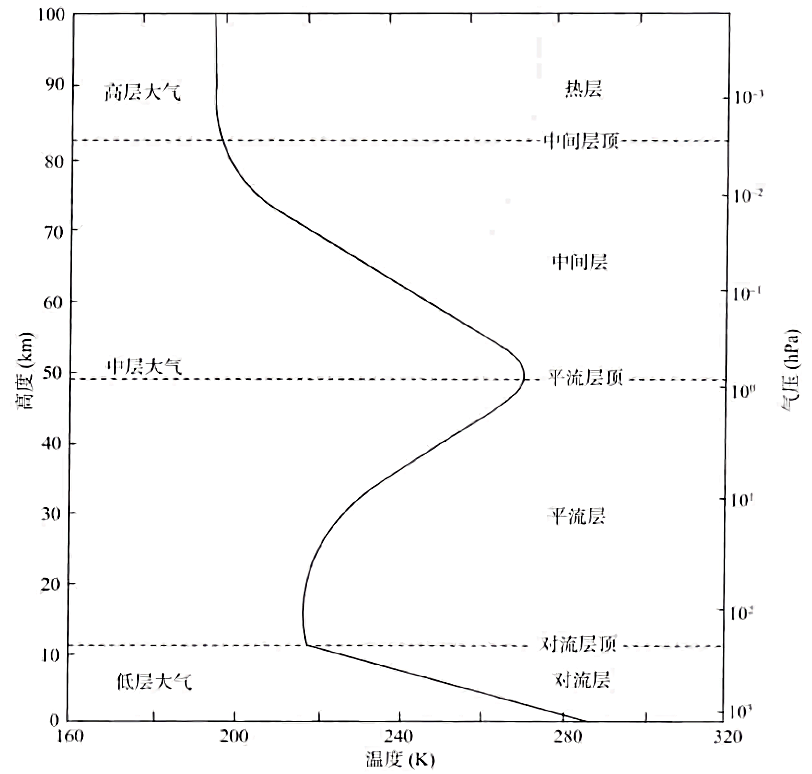
\includegraphics[height=0.9\textwidth]{大气垂直温度轮廓线和分层1.png}
    \caption{大气垂直温度轮廓线和分层}
    %\label{fig:logo}
    %\note{注:图注的内容不宜放到图题中。}
\end{figure}
地面以上大气的最底层称为对流层,对流层顶的高度约为10km,气压约为200hPa。
对流层集中了大气质量的75$\%$
以上,几乎全部云、水汽和降水,主要天气现象,如台风、寒潮和雷电等,都发生在这层。
温度随高度升高而降低是对流层的主要特征,大约每升高1 km降低6.5$^\circ C$。

对流层顶向上到50km左右的这一层为平流层,平流层顶的气压约为1 hPa。 
平流层下部温度随高度变化很小,平流层上部因为存在臭氧层,
臭氧吸收太阳紫外辐射使大气温度增加,这种上部热下部冷的逆温结构平流层大气很稳定,
空气大多做水平运动。
平流层顶到85 km左右称为中间层,中间层顶气压约0.01 hPa,中间层大气温度随高度递减,
水汽极少,有相当强的垂直混合,60 km以上大气分子开始电离,电离层的底部就在中间层内。
中间层顶以上到500 km的这一层称为热层。由于热层的分子氧和原子氧能吸收太阳紫外辐射和微粒辐射,
所以这一层温度又随高度升高而增加,很难有对流运动,造成巨大温度梯度和昼夜温差。

在构成大气的气体中,氮气($N_2$)和氧气($O_2$)约占99$\%$,
氩气($Ar$)、水汽($H_20$)、二氧化碳($CO_2$)、臭氧($O_3$)及其他气体($H_20$,$CH_4$,$NH_4$等)约占1$\%$,
图3.2给出了主要吸收气体的垂直分布廓线。大气中还包含各种气溶胶等微粒。
气溶胶是一种固体、液体的悬浮物,由尘埃、盐粒等组成一个核心,在核心以外包有一层液体。

\begin{figure}[htb]
    \centering
    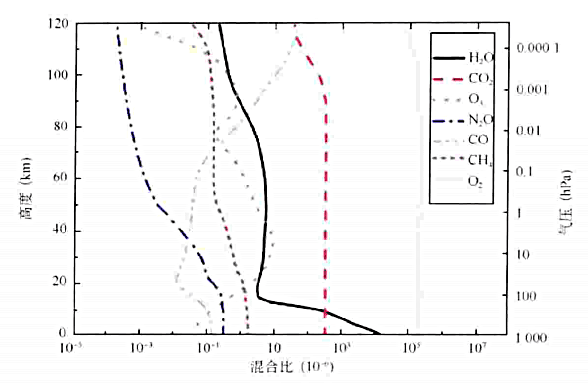
\includegraphics[height=0.6\textwidth]{不同气体的垂直分布廓线1.png}
    \caption{不同气体的垂直分布廓线}
    %\label{fig:logo}
    %\note{注:图注的内容不宜放到图题中。}
\end{figure}

气体分子对不同波长的辐射有强烈而复杂的吸收光谱,图3.3为主要吸收气体的光谱分布图。
对流层中,水汽是最重要的吸收气体,其次是$CO_2$;平流层中,$H_20$,$CO_2$和$0_3$的吸收作用相当;
中间层大气中的主要吸收气体是$CO_2$。

\begin{figure}[htb]
    \centering
    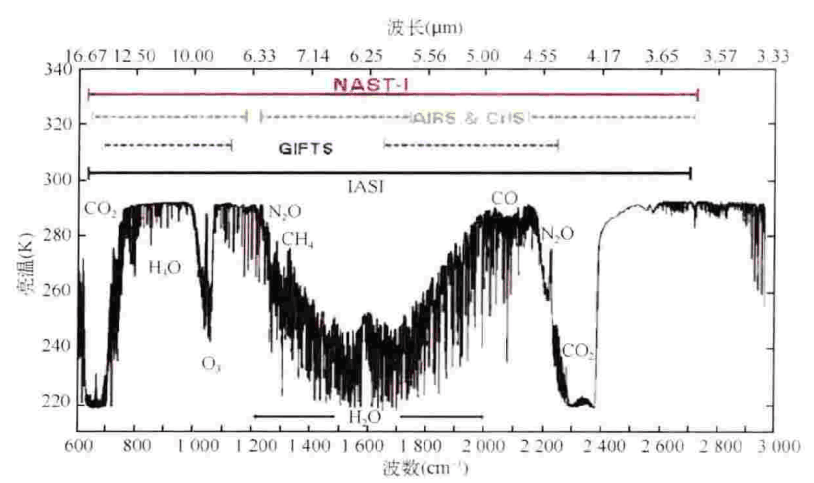
\includegraphics[width=\textwidth]{不同气体的吸收光谱.png}
    \caption{不同气体的吸收光谱}
    %\label{fig:logo}
    %\note{注:图注的内容不宜放到图题中。}
\end{figure}

多通道扫描成像辐射计是风云四号的载荷之一,
通过精密的双扫描镜机构实现灵活和精确的二维指向,
可实现分钟级的快速区域扫描;采用离轴三反主光学系统,高频次获取十四波段的地球云图,
利用星上黑体,进行高频次红外定标,确保了观测数据的精度\cite{FY4A}。

多通道扫描成像辐射计主要负责获取云图的任务,共十四个通道,是风云二号五通道的近三倍,
在风云二号观测水汽、云、地表和植被的基础上,还具备了捕捉雪和气溶胶的能力,
并且能清晰区分云的不同相态和中高层水汽。与风云二号单一可见光通道相比,
风云四号可以制作出彩色卫星云图,1分钟即可生成一次区域观测图像。成像仪的主要技术指标如表3.1所示。

\begin{table}[htb]
    \centering\small
    \caption{多通道扫描辐射计主要技术指标}
    \label{tab:exampletable}
    \begin{tabular}{ll}
      \toprule
        技术指标   & 指标参数     \\
      \midrule
      搭载卫星 & FY-4A \\
      重量 & 306Kg   \\
      通道数量 & 14个(6个可见/近红外波段,2个中波红外波段, \\
       & 2个水汽波段和4个长波红外波段)       \\
      空间分辨率 & 可见/近红外波段为0.5$\sim$1Km,红外波段为2Km$\sim$4Km     \\
      全圆盘扫描时间 & 15分钟  \\
      区域扫描时间 & 1分钟(1000Km$\times$1000Km)  \\
      \bottomrule
    \end{tabular}
  \end{table}

  \begin{table}[htb]
    \centering\small
    \caption{多通道扫描辐射计主要技术指标}
    \label{tab:exampletable}
    \begin{tabular}{cllll}
      \toprule
        通道序号 & 通道类型 & 中心波长  & 空间分辨率 & 主要用途    \\
      \midrule
      1 & 可见光与近红外 & $0.45\mu m$  & 1Km & 小粒子气溶胶 \\
      2 &  & 0.65$\mu m$ & 0.5Km$\sim$1Km & 植被 \\
      3 &  & 0.82$\mu m$ &  1Km & 植被,水面上气溶胶 \\
      4 & 短波红外 & 1.37$\mu m$ & 2Km & 卷云 \\
      5 &  & 1.61$\mu m$  & 2Km & 低云/雪识别 \\
      6 &  & 2.25$\mu m$ & 2Km$\sim$4Km & 卷云、气溶胶 \\
      7 & 中波红外 & 3.75$\mu m$ & 2Km & 云等高反照率目标 \\
      8 &  & 3.75$\mu m$ & 4Km & 低反照率目标,地表 \\
      9 & 水汽 & 6.25$\mu m$  & 4Km & 高层水汽 \\
      10 &  & 7.1$\mu m$  & 4Km & 中层水汽 \\
      11 & 长波红外 & 8.5$\mu m$  & 4Km & 总水汽\\
      12 &  & 10.7$\mu m$  & 4Km & 云、地表温度等 \\
      13 &  & 12.0$\mu m$  & 4Km & 云、总水汽量\\
      14 &  & 13.5$\mu m$ & 4Km & 云、水汽 \\
      \bottomrule
    \end{tabular}
  \end{table}
  
成像仪各通道性能参数如表3.2所示。可以观察到,序号低的通道(波长短)主要观测近地气溶胶及低云,
序号高的通道(波长长)主要观测中高层水汽。根据雷暴云的物理特性,雷暴成熟时云顶高度高,中高层云聚集大量水汽,
可知在中长波红外和水汽通道能够较好反映出雷暴信息。


\section{雷暴尺度及强度问题}
雷暴是由强对流生成的,
由水平尺度几千米到十几千米的雷暴单体的积雨云所组成,有雷电活动的单体寿命约为30分钟到1小时。
闪电率可以从每分钟不足一次到每分钟十次以上,通常在第一次闪电之后大约10$\sim$20 min内出现最大的闪电。
在单体整个生存期内,平均闪电率约为每分钟2至3次,但是雷暴是由多个单体组成,对整个雷暴而言,
平均闪电率约为每分钟3至4次。

本文所采用的风云四号数据为成像仪全圆盘4KML1级数据,该数据包含扫描辐射成像计14个通道的云图信息,
云图分辨率为4km。在建立样本库时,将会从不同通道提取出不同宽度的正方形云图,
根据雷暴云的物理特性,可以计算出样本库单个云图应取50个像素值左右,若取值过多,则超过雷暴云的尺度范围,
将会包含更多无效信息;若取值过少,将无法提取出雷暴云的图像特征。

风云四号的闪电数据由卫星上搭载的闪电成像仪提供,闪电成像仪采用CCD面阵和光学成像技术,
对观测区域内包括云闪、云地闪和云间闪在内的总闪电进行凝视观测,实现对雷暴系统的实时、
连续监测和跟踪,为强对流天气监测、铁路、电力和民航等行业安全保障等提供服务\cite{fengyunsihao}。
闪电成像仪主要技术指标如表3.3所示。

\begin{table}[htb]
    \centering\small
    \caption{闪电成像仪主要技术指标}
    \label{tab:exampletable}
    \begin{tabular}{ll}
      \toprule
        技术指标   & 指标参数     \\
      \midrule
      搭载卫星 & FY-4A \\
      重量 & 65Kg   \\
      尺寸 &  528mm(长)$\times$346mm(宽)$\times$1032mm(高)\\
      CCD面阵 &  400$\times$600单元\\
      成像速率 & 500帧/秒  \\
      中心波长 & 777.4nm \\
      带宽 & 1nm \\
      空间分辨率 & 7.8Km@星下点 \\
      总视场角 & 4.98$\circ$(南北)$\times$7.41$\circ$(东西)\\
      闪电探测率 & 90$\%$  \\
      虚警率 & 10$\%$ \\
      \bottomrule
    \end{tabular}
  \end{table}

闪电成像仪 CCD 面阵利用 777.4 nm近红外通道探测发光事件,经星上实时事件处理器进行背景光评估,输出经背景光
滤除后的发光事件的强度和位置等信息,通过聚类滤除算法将发光事件聚类为“事件”,“组”和“闪电”产品,
包括“事件”,“组”和“闪电”的位置、强度和发生时间等信息。处理过后以闪电仪1分钟组产品的方式发送给用户,
该产品为NC格式的数据,存储有“闪电组”的经纬度,时间,强度等信息,其中GEC(Group Event Count)
存储了闪电的强度信息,闪电强度越大,对应位置的雷暴云图特征将更为明显\cite{lmi}\cite{shandianyi}。


\section{特征融合问题}
本文选用灰度共生矩阵的方法计算出角二阶矩、对比度、逆差距和熵等四种纹理特征量化值,几何特征方面选取了云区
面积、质心、偏心率等特征,数据分析中多维的数据往往很难找出准确的特征,
因此本文将采用主成分分析的方法来分析和简化数据。

在多元统计分析中,主成分分析(Principal components analysis,PCA)
可以用来降低数据集的维数,同时保留数据集中对方差贡献最大的特征。
这是通过忽略高阶主成分,保留低阶主成分做到的,
由于主成分分析过于依赖所给数据,所以对数据的准确性要求很高。

主成分分析由卡尔·皮尔逊于1901年发明,用于建立数理模型和分析数据。
其方法主要是通过对协方差矩阵进行特征分解,以得出数据的主成分(即特征向量)与它们的权值(即特征值)。
PCA是最简单的以特征量分析多元统计分布的方法。 结果可以理解为数据值对方差影响最大的方向。
PCA提供了一种减少数据维度的有效方法,如果从原始数据中移除对应于最小特征值的分量,
所得到的低维数据就是优化过的,在分析复杂数据时,主成分分析特别有用。

PCA是以特征量分析多元数据统计分布的方法。通常情况下,这种运算可以被看作是一种揭露数据的内部结构,
从而更好的解释数据变量的方法。如果多元数据集能够在一个高维数据空间坐标系中被表示出来,
那么PCA就能够计算出一幅比较低维度的图像,这幅图像即为在信息最多的点上原对象的一个‘投影’。
这样就可以利用少量的主成分来降低数据的维度。

遥感图像处理中一幅多波段遥感图像的不同波段之间往往存在着很高的相关性,
对其进行主成分变换的实质是将具有相关性的多波段数据压缩到完全独立的较少的几个波段上,
使新图像数据更易于解译。将不同时相的多波段数据经主成分变换后,
新图像中各主分量正交即各主分量之间的相关系数为零或接近零。
一般来说,第一主分量包括了原始多波段影像信息的绝大部分内容,相当于原来各波段的加权和,
每个波段的权值与该波段的方差大小成正比,其他各主分量所包括的信息逐渐减少。
主成分分析的优点在于降低各波段的相关性,较好地保留影像的纹理并突出不同的地物目标,
不限制变换的波段的数量。其缺点是变换后每一主分量所突出的信息有所不同,需要靠经验来进行选择\cite{zhuchengfen}。

\section{小结}
本章首先从传感器波段角度,分析了风云四号卫星搭载的多通道扫描成像辐射计各波段参数,
选取出中长波红外和水汽通道作为雷暴云特征提取的主要通道;之后根据雷暴的物理尺度和强度,
分析了样本库云图数据的分辨率,大致应在50个像素值左右,雷暴强度越强特征则会越明显;
最后从特征融合的角度,选取主成分分析方法来进行数据降维,以便分析提取出更为准确的信息。
本章尝试从理论方面进行了分析,第五章则会通过建立好的样本库进行测试验证。
% !TeX root = ../main.tex

\chapter{样本库的建立及数据分析}
特征提取需要大量样本才能提取出相对准确的信息,对于不同类型的数据也有不同的分析方法,
本章主要介绍研究过程中样本库的建立过程以及数据分析方法,流程图如图4.1所示。
\begin{figure}[htb]
    \centering
    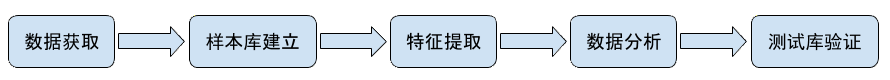
\includegraphics[width=\textwidth]{特征提取流程图.png}
    \caption{样本库的建立及数据分析流程图}
    %\label{fig:logo}
    %\note{注:图注的内容不宜放到图题中。}
\end{figure}

\section{云图数据的获取和分类}
本文数据全部来自于我国第二代静止气象卫星,风云四号气象卫星(FY4A星),该星装载多种观测仪器,
包括多通道扫描成像辐射计、闪电成像仪、空间环境监测仪器和干涉式大气垂直探测仪等仪器。
FY4A提供各个观测仪器的L1级数据,包括成像仪500M,1KM,2KM,4KM等不同分辨率全圆盘数据,
闪电仪1分钟组产品等。FY4A还提供了32种定量产品,包括云和大气产品、地表类产品、天气产品、
辐射产品等多种种类,大气的相关信息可以由大气类产品来监测,环境监测主要用地表类产品,
环境灾害天气的监测则主要使用天气类产品,地气系统辐射收支情况则用辐射类产品来反映。

本文实验数据来自于中国气象局国家卫星气象中心,可通过风云卫星遥感数据服务网下载卫星数据。
经过分析比较最终选取了成像仪全圆盘4KML1数据,闪电仪1分钟组产品和云检测实时产品,
其中成像仪全圆盘4KML1数据用于提取$0.45\sim13.8\mu m$等14个通道的云图数据,
闪电仪1分钟组产品用于建立雷暴云数据库,云检测实时产品用于建立非雷暴云数据库。

在风云卫星遥感数据服务网选取数据提交订单后,由国家气象卫星中心回调所需数据,
回调完成将返回下载数据所需的用户名和密码,在个人服务器端通过FTP即可进行下载。
下载完成后的成像仪全圆盘数据为HDF格式,闪电仪组产品和云检测产品为NC格式,为方便后续处理,
根据文件名将不同数据分类保存至对应文件夹。成像仪和云检测产品的数据以一小时为间隔,
闪电仪的数据以一分钟为间隔,为了将闪电仪数据和成像仪数据相匹配,
本文选取成像仪数据时间后十分钟闪电仪数据,
保存至对应文件件。分类后的文件格式如图4.2:
\begin{figure}[htb]
    \centering
    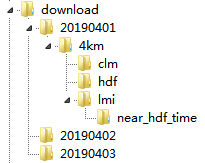
\includegraphics[width=0.4\textwidth]{分类后文件格式.png}
    \caption{分类后文件格式}
    %\label{fig:logo}
    %\note{注:图注的内容不宜放到图题中。}
\end{figure}

其中download表示下载的数据,下级目录20190401表明数据时间,下级目录4km表明数据分辨率为4km,
其中clm中存放云检测产品数据,hdf中存放成像仪全圆盘数据,lmi中存放闪电仪数据,
near$\_$hdf$\_$time文件夹单独存放临近成像仪数据时间的闪电仪数据。


\section{样本库的建立}
本文需要分析大量分析,才能得出相对准确的结果,因此样本库的建立是非常重要的一步,将根据闪电仪数据和
云检测产品建立雷暴云样本库和非雷暴云样本库,为之后的特征提取分析奠定基础。

\subsection{雷暴云样本库的建立}
雷暴云样本库的建立需要闪电仪数据作为已知信息,闪电成像仪是全球第一批两颗静止气象卫星闪电成像仪之一,
我国首次研制,采用CCD面阵和光学成像技术,对观测区域内包括云闪、云间闪、云地闪在内的总闪电进行凝视观测,
实现对雷暴系统的实时、连续监测和跟踪。数据以NC格式存储,其中存储着一次闪电事件的经纬度,辐射强度,
发生时间等信息,为方便后续处理,提取所有闪电信息并保存为csv文件,文件如图4.3所示:

\begin{figure}[htb]
    \centering
    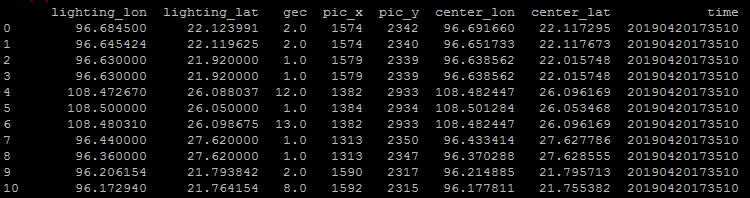
\includegraphics[width=\textwidth]{存储闪电信息的csv文件.png}
    \caption{存储闪电信息的csv文件}
    %\label{fig:logo}
    %\note{注:图注的内容不宜放到图题中。}
\end{figure}


每一行表示一次闪电事件,lighting$\_$lon表示闪电实际发生的经度,lighting$\_$lat表示闪电实际发生的纬度,
gec表示闪电的强度(标准化后的数值,与实际闪电辐射强度成正比),pic$\_$x,pic$\_$y,center$\_$lon,center$\_$lat
分别表示闪电对应在hdf卫星云图上的行列值,以及对应的经纬度
(由于hdf云图中没有经纬度数据,只能通过官方文档《FY-4A数据行列号和经纬度查找表4km》查表计算),
time表示闪电发生的时间,依次为年月日时分秒。

根据闪电仪csv中数据即可从成像仪hdf数据中提取出各通道对应的卫星云图,
首先根据time闪电时间信息找到对应时间的hdf数据,接着根据pic$\_$x和pic$\_$y即闪电对应hdf数据行列号,
设置不同分辨率(以行列号为中心)即可提取出不同通道的雷暴云图像。最终生成的文件树如图4.4。

\begin{figure}[htb]
    \centering
    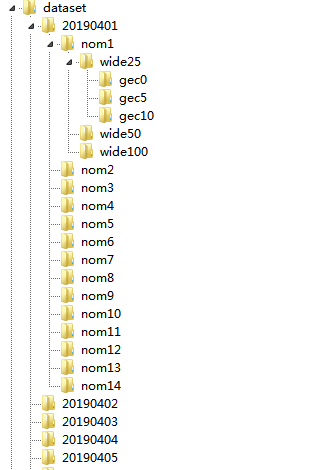
\includegraphics[height=0.5\textwidth]{雷暴云数据库文件格式.png}
    \caption{雷暴云数据库文件格式}
    %\label{fig:logo}
    %\note{注:图注的内容不宜放到图题中。}
\end{figure}

dataset表示数据库,20190401表示数据库年月日,nom1~14表示全圆盘4KM数据14个通道数据
,$wide25$,$wide50$,$wide100$表示生成云图的分辨率(即像素值),
gec5表示雷暴强度为$5\sim10$的数据集,gec10表示雷暴强度为$10\sim15$的数据集。

根据官方文档可知,云图数据以辐射值存储,变化范围为0$\sim$65534,其中65535为无效值,
因此在处理时,将65535变为0,将0$\sim$65535压缩到0$\sim$255,调用opencv相关函数生成云图图像。
生成的雷暴云图如图4.5。


\iffalse
\begin{figure}[htb]
\centering
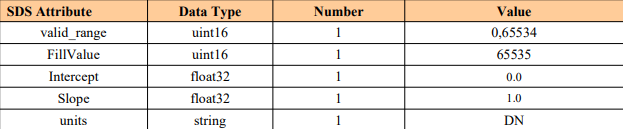
\includegraphics[width=\textwidth]{云图图像数据层数据官方文档.png}
\caption{云图图像数据层数据官方文档}
%\label{fig:logo}
%\note{注:图注的内容不宜放到图题中。}
\end{figure}
\fi


\begin{figure}[htb]
    \centering
    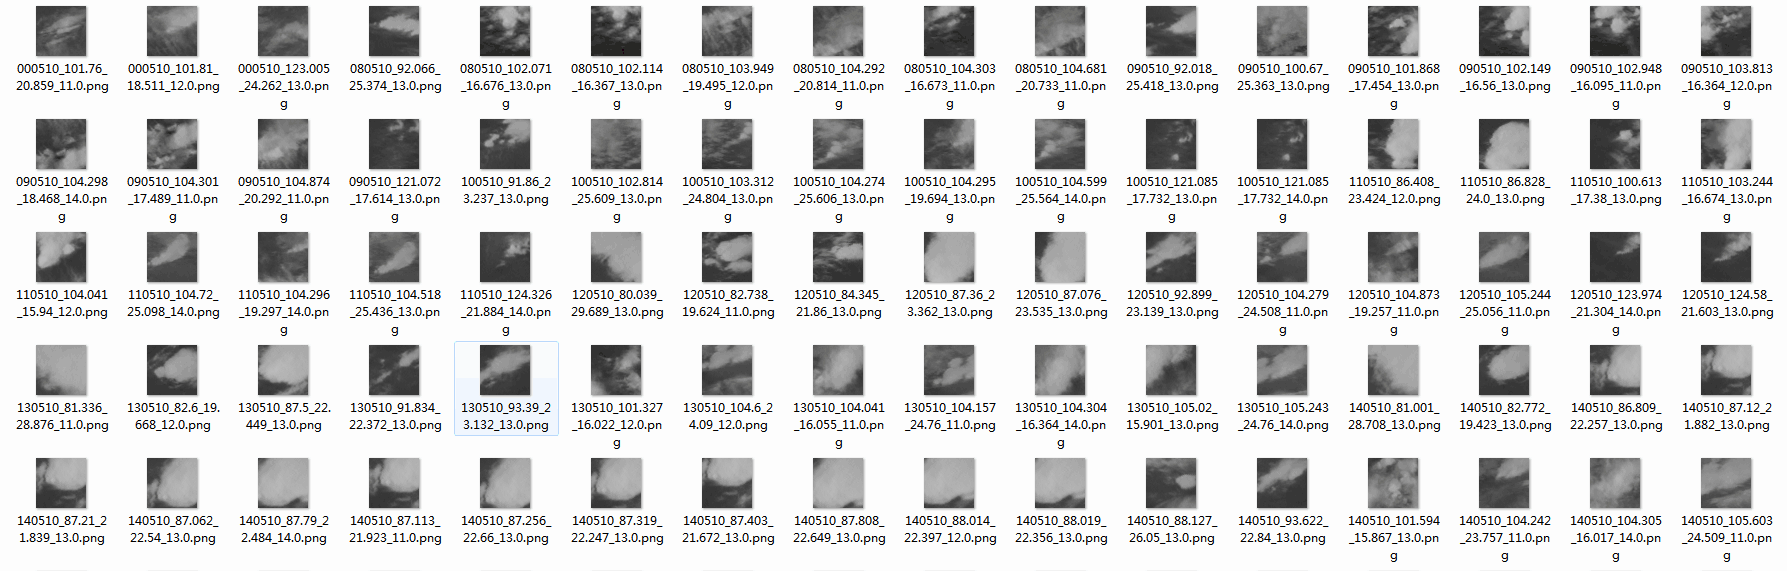
\includegraphics[width=\textwidth]{生成的雷暴云图像2.png}
    \caption{生成的雷暴云图像}
    %\label{fig:logo}
    %\note{注:图注的内容不宜放到图题中。}
\end{figure}


\subsection{非雷暴云样本库的建立}
非雷暴云样本库的建立需要云检测产品作为已知信息,风云四号云检测产品处理是联合利用多通道
扫描成像仪的多个通道,采用阈值法,经过处理,生成的云检测产品。云检测产品中填充值0表示为云,1表示可能为云,2表示可能晴空,3表示晴空,126表示地表之外的空间,127表示无效值。
不同分辨率下某一区域平均值小于一定阈值,即可将此区域判定为云,
选取示意图如图4.6所示。
\begin{figure}[htb]
    \centering
    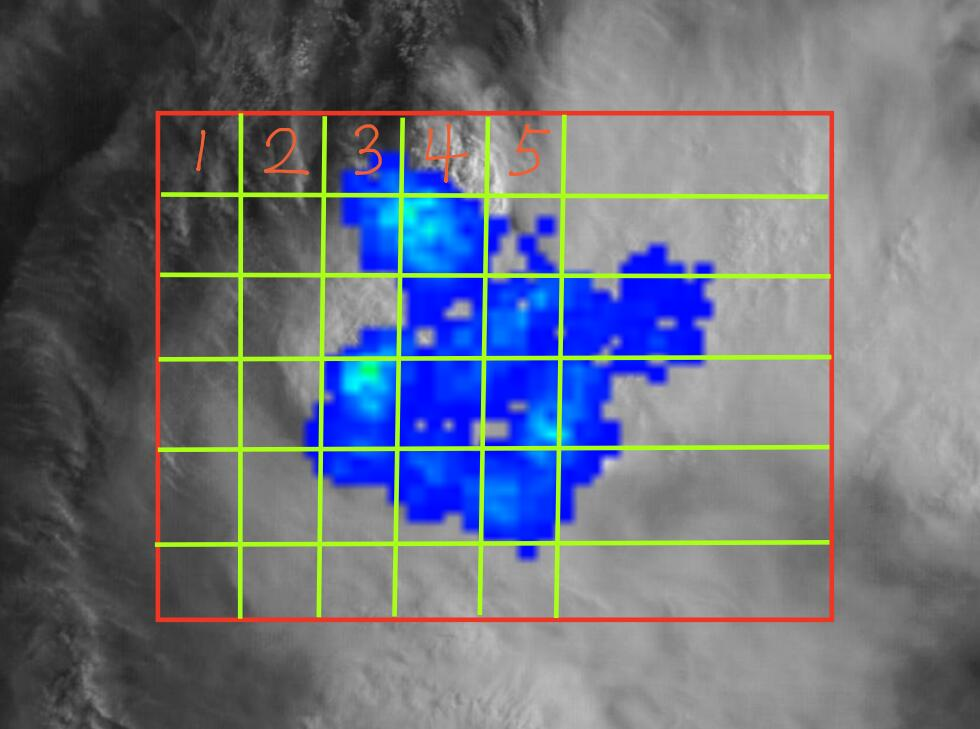
\includegraphics[height=0.5 \textwidth]{非雷暴区域选定示意图.jpg}
    \caption{非雷暴区域选定示意图}
    %\label{fig:logo}
    %\note{注:图注的内容不宜放到图题中。}
\end{figure}



以一定分辨率划定区域,本文假定划定区域平均值小于0.01即判断为云,
则此实例中1,2判定为非云区,3,4,5区域可判定为云区,其中3,4区域由于有闪电仪数据,
因此只有5区域判定为非云区,
将生成的云图图像保存至对应通道对应分辨率的gec0文件夹中,表示雷暴强度为0。
生成的部分非雷暴云图如图4.7。文件名分别表示时间和经纬度。
\begin{figure}[htb]
    \centering
    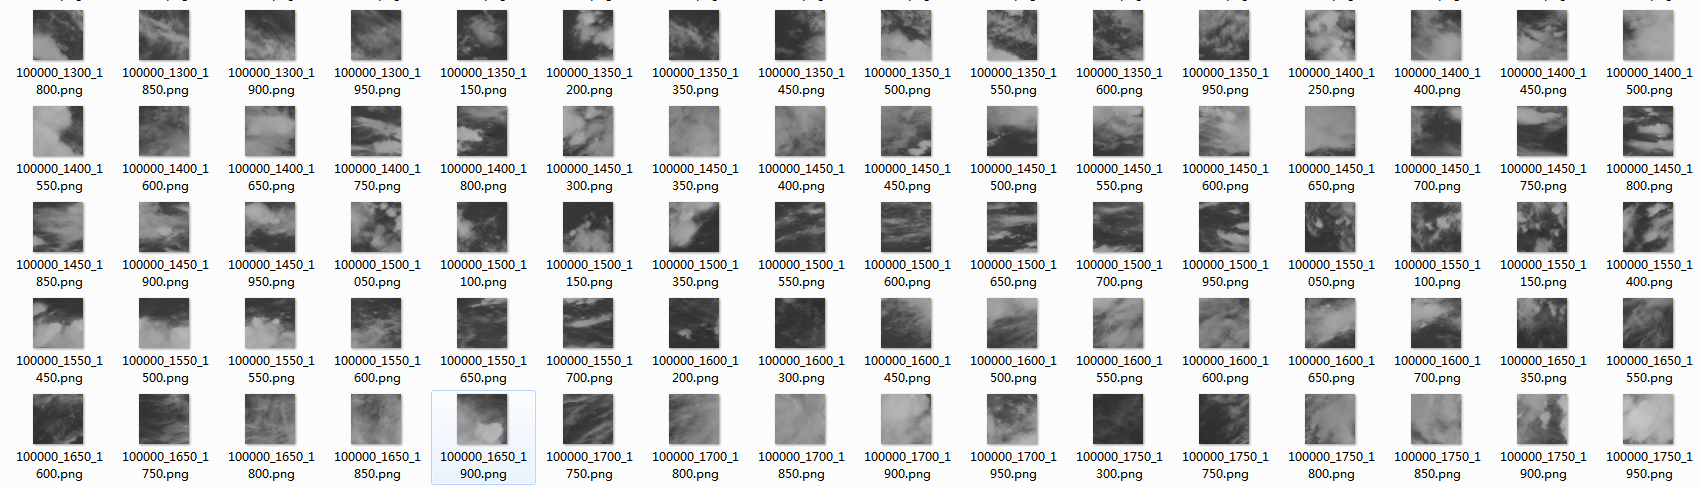
\includegraphics[width=\textwidth]{部分非雷暴云图.png}
    \caption{部分非雷暴云图}
    %\label{fig:logo}
    %\note{注:图注的内容不宜放到图题中。}
\end{figure}


\section{图像的特征提取}

\subsection{纹理特征提取}
本文采用灰度共生矩阵的方法对图像的纹理特征进行计算,
挑选了ASM,CON,IDM,ENG等四个量值进行图像的分类。
如果影像中噪声越多,则ASM能量值就越小,代表影像纹理越丰富。
如果影像中地物灰度分布均匀(例如,云层、水体),则ASM能量值越大,纹理信息越弱。
对比度(CON)描述的是影像中像素与其周围像素的反差对比。
对比度越小,说明该区域的像素灰度越均匀,纹理越弱,反之,纹理越丰富。
IDM是反映图像中某一区域内像元值变化程度的量。IDM值越大,说明图像中该区域的纹理越弱,
反之,纹理越丰富。熵原本用来描述分子不规则运动剧烈程度的物理量,
后来用来度量影像中所包含的纹理信息。熵值越大,说明影像中所包含的纹理信息越丰富,
反之,纹理信息越弱。计算得到的四种纹理特征量值如图4.8所示。

\begin{figure}[htb]
    \centering
    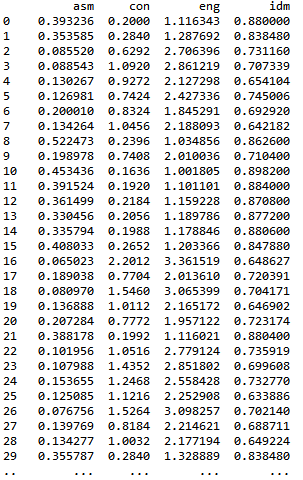
\includegraphics[width=0.5\textwidth]{计算得到的纹理特征量值.png}
    \caption{计算得到的纹理特征量值csv存储方式}
    %\label{fig:logo}
    %\note{注:图注的内容不宜放到图题中。}
\end{figure}

\iffalse
\begin{algorithm}[htb]
    \small
    \SetAlgoLined
    \KwData{this text}
    \KwResult{how to write algorithm}
  
    initialization\;
    \While{not at end of this document}{
      read current\;
      \eIf{understand}{
        go to next section\;
        current section becomes this one\;
      }{
        go back to the beginning of current section\;
      }
    }
    \caption{纹理特征计算算法}
    \label{algo:algorithm1}
\end{algorithm}
\fi

\newpage
\subsection{几何特征提取}
卫星云图上的各类云系都具有一定的边界形状,云的边界是判断天气系统的重要依据,如成熟的台风呈圆形,
冷锋云带呈气旋形弯曲。形状的描述主要分为以下几种方法:基于面积、伸长度、主轴方向等传统的形状特征;
基于形状变换的方法;基于形状相互关系的方法。本文主要从图形的周长,面积,等效直径,离心率等方面来描述形状特征。

首先通过阈值法提取出云图的二值图像,之后通过形态学的方法计算出图像的连通区域,不同区域标记为不同的颜色,
如图4.9所示。
\begin{figure}[htb]
    \centering
    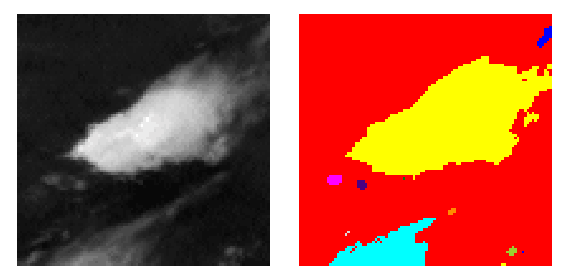
\includegraphics[width=0.9\textwidth]{阈值法处理后的云图区域.png}
    \caption{阈值法处理后的云图区域}
    %\label{fig:logo}
    %\note{注:图注的内容不宜放到图题中。}
\end{figure}
此图共提取出12块连通区域,可看出标记为黄色的连通区域表示此图中主要的云图信息,因此只需保留此块区域的几何特征,
通过计算各连通区域的面积,得出最大面积的连通区域即为此区域,计算此区域不同的几何特征,
将计算后的几何特征以csv的格式保存,如图4.10所示。
\begin{figure}[htb]
    \centering
    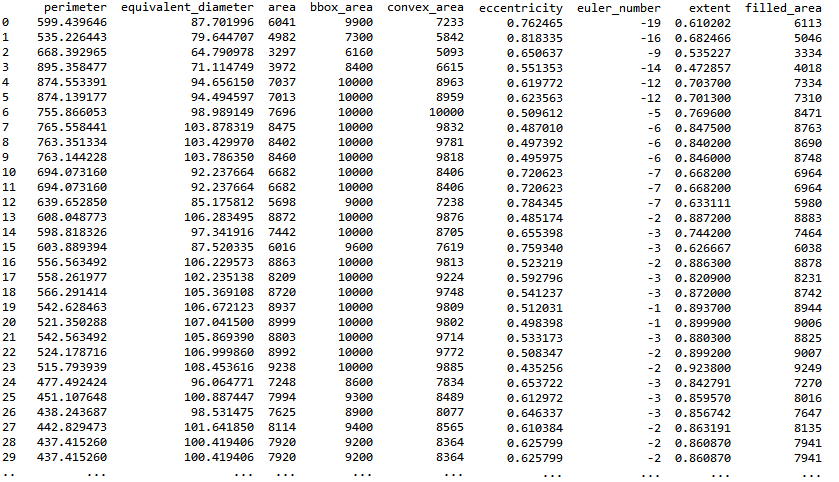
\includegraphics[width=\textwidth]{计算得到的几何特征.png}
    \caption{计算得到的几何特征csv存储方式}
    %\label{fig:logo}
    %\note{注:图注的内容不宜放到图题中。}
\end{figure}

perimeter表示区域周长,equivalent$\_$diameter表示等效直径(和区域面积相同的
圆的直径),area表示区域面积,bbox$\_$area表示边界外接框的面积,convex$\_$area表示凸包的
面积,eccentricity表示离心率,euler$\_$number表示欧拉数,extent表示区域面积和边界外接框面积的比率,
filled$\_$area区域和外接框之间填充的面积。

\iffalse
\subsection{频率特征提取}
影像频率是描述影像中光谱信息变化程度的的物理量。对于影像中的云层而言,
云层边缘灰度突变,因此分布在高频部分,
而云层内部灰度均匀,因此分布在低频部分。频率域为评价影像提供了一个全新的角度。
本文通过快速傅里叶变换,计算得出云图图像的幅度谱如图。

\begin{figure}[htb]
    \centering
    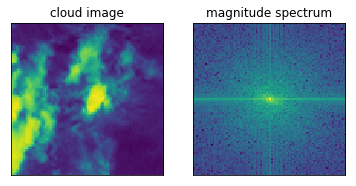
\includegraphics[width=0.5\textwidth]{卫星云图和FFT变换后的幅度谱.png}
    \caption{卫星云图和FFT变换后的幅度谱}
    %\label{fig:logo}
    %\note{注:图注的内容不宜放到图题中。}
\end{figure}
\fi


\section{特征数据的分析}
\subsection{纹理特征的分析}
4.3.1中提取到的ASM,CON,IDM,ENG等四个量值以CSV格式保存,由于数据维度并不高,不必采用主成分分析的方法
降维处理,在分析时通过比较不同分辨率,
不同雷暴强度 ,不同波段,不同的纹理特征组合,确定出区分雷暴云和非雷暴云的阈值范围,
主要采用散点图的方式进行数据可视化,x轴表示其中一种纹理特征值,y轴表示另一种纹理特征值,
将要比较的两幅图像叠加在一幅图像上,即可较为清晰的看出是否具有可靠的区分度。

第一幅图表示1通道分辨率为25像素雷暴强度为5以及1通道分辨率为50像素雷暴强度为5的asm值和con值的组合,
可看出不同分辨率的图像区分度并不高。第二幅图表示10通道分辨率为25像素雷暴强度为0(即非雷暴区域)
以及10通道分辨率为25像素雷暴强度为10的eng值和idm值的组合,具有较高的区分度。
关于纹理特征的详细分析,将重点在第五章进行讨论。

\begin{figure}[htbp]
\centering
\begin{minipage}[t]{0.48\textwidth}
\centering
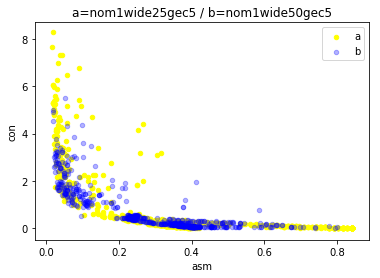
\includegraphics[width=6cm]{纹理特征分析方法1.png}
\caption{纹理特征分析方法1}
\end{minipage}
\begin{minipage}[t]{0.48\textwidth}
\centering
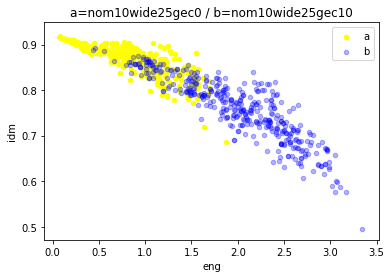
\includegraphics[width=6cm]{纹理特征分析方法2.png}
\caption{纹理特征分析方法2}
\end{minipage}
\end{figure}
    
\subsection{几何特征的分析}
\subsubsection{主成分分析方法}
4.3.2中提取到的纹理特征,共有周长、直径、面积等九个数据维度,
在分析时采用主成分分析的方法来降低数据维度。
主成分分析主要分为以下几步:

(1)对数据进行标准化处理;

(2)计算标准化后的协方差矩阵;

(3)计算协方差矩阵的特征值及特征向量;

(4)各成分贡献率并按大小排列;

(5)根据主成份贡献率的大小选取前m个主成份;

(6)将原始数据与对应的特征向量矩阵相乘即可得到降维后的数据。

经过计算得出的各分量贡献率如表4.1所示。

\begin{table}[htb]
    \centering\small
    \caption{主成分分析各分量贡献率}
    \label{tab:exampletable}
    \begin{tabular}{cllll}
      \toprule
        component & value & difference  & proportion & cumulative    \\
      \midrule
      1 & 6.3139 & 4.5995 & 0.7015 & 0.7015 \\
      2 & 1.7143 & 1.2567 & 0.1904 & 0.8920 \\
      3 & 0.4575 & 0.0877 & 0.0508 & 0.9428 \\
      4 & 0.3698 & 0.2487 & 0.0411 & 0.9839 \\
      5 & 0.1211 & 0.1083 & 0.1346 & 0.9974 \\
      6 & 0.0128 & 0.0039 & 0.0014 & 0.9988 \\
      7 & 0.0089 & 0.0077 & 0.0009 & 0.9998 \\
      8 & 0.0011 & 0.0007 & 0.0001 & 0.9999 \\
      9 & 0.0004 & 0 & 0.0001 &  1\\
      \bottomrule
    \end{tabular}
  \end{table}

由表4.1可以看出1,2分量累积贡献率已接近90$\%$,由1,2分量对应的特征向量
构成的特征矩阵,可以计算得出降维后的数据。由于采用了两个分量,
因此可以采用散点图的方式来表示数据,将雷暴云和非雷暴云的几何特征
降维后放在一张散点图中如图4.13所示。

\begin{figure}[htb]
    \centering
    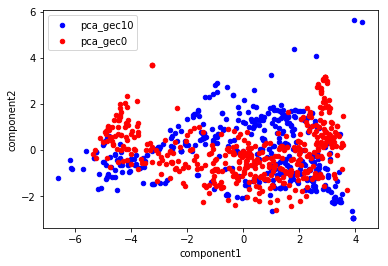
\includegraphics[width=0.8\textwidth]{降维后的几何特征分析.png}
    \caption{降维后的几何特征分析}
    %\label{fig:logo}
    %\note{注:图注的内容不宜放到图题中。}
\end{figure}

\subsubsection{密度图分析方法}
将计算出的不同的几何特征值用密度图来表示,可以看出不同特征值大致的分布,
每幅图下方标明此图对比的几何特征名称,
蓝色的线表示雷暴强度大于10的雷暴云对应的密度曲线,
红色的线表示非雷暴云对应的密度曲线。如图4.14所示。
\begin{figure}
    \centering
    \subfigure{
    \begin{minipage}[t]{0.25\linewidth}
    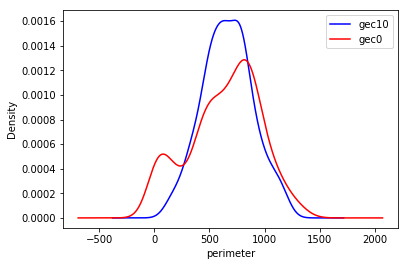
\includegraphics[width=1\linewidth,height=0.7\linewidth]{311.png}\vspace{2pt}
    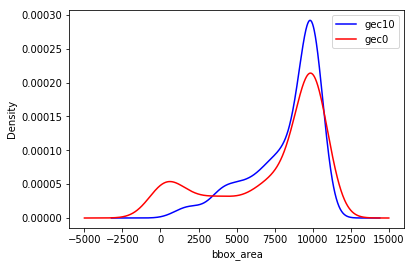
\includegraphics[width=1\linewidth,height=0.7\linewidth]{314.png}\vspace{2pt}
    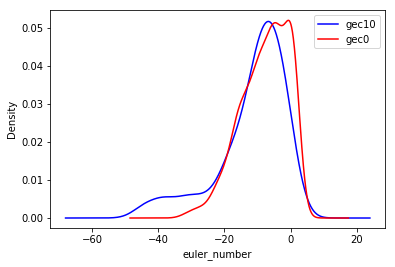
\includegraphics[width=1\linewidth,height=0.7\linewidth]{317.png}
    \end{minipage}}
    \subfigure{
    \begin{minipage}[t]{0.25\linewidth}
    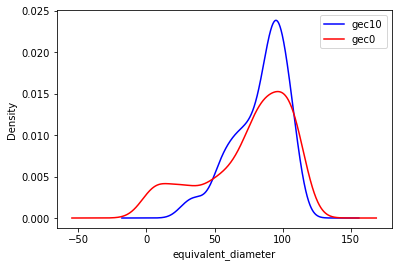
\includegraphics[width=1\linewidth,height=0.7\linewidth]{312.png}\vspace{2pt}
    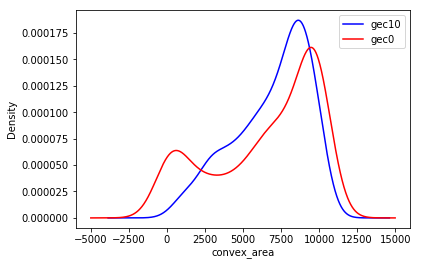
\includegraphics[width=1\linewidth,height=0.7\linewidth]{315.png}\vspace{2pt}
    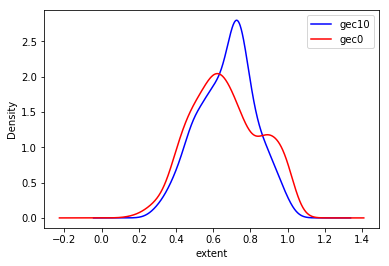
\includegraphics[width=1\linewidth,height=0.7\linewidth]{318.png}
    \end{minipage}}
    \subfigure{
    \begin{minipage}[t]{0.25\linewidth}
    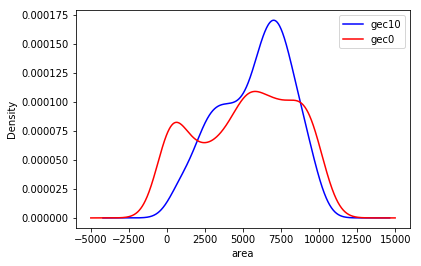
\includegraphics[width=1\linewidth,height=0.7\linewidth]{313.png}\vspace{2pt}
    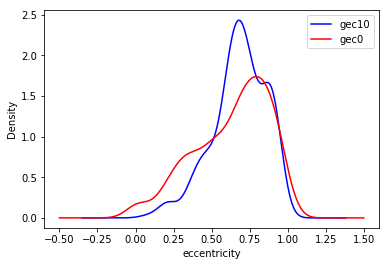
\includegraphics[width=1\linewidth,height=0.7\linewidth]{316.png}\vspace{2pt}
    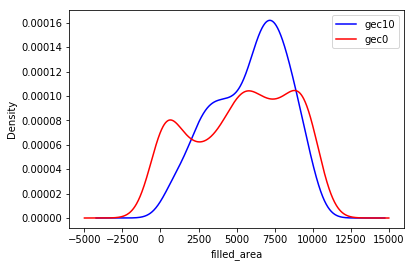
\includegraphics[width=1\linewidth,height=0.7\linewidth]{319.png}
    \end{minipage}}
    \caption{不同几何值的密度图}
    \end{figure}

perimeter表示区域周长,equivalent$\_$diameter表示等效直径(和区域面积相同的
圆的直径),area表示区域面积,bbox$\_$area表示边界外接框的面积,convex$\_$area表示凸包的
面积,eccentricity表示离心率,euler$\_$number表示欧拉数,extent表示区域面积和边界外接框面积的比率,
filled$\_$area区域和外接框之间填充的面积。
可以看出雷暴云和非雷暴云在各个特征值下,分布都非常接近,不能准确区分雷暴云和非雷暴云。

\section{测试库的建立和验证}
测试库的建立与样本库的建立方法类似,将提取到的雷暴云和非雷暴云放在一个文件夹中。
根据本文提出的图像特征阈值提取方法进行判别,为了对该方法进行定量化分析,
研究中引入了预警率、虚警率以及错误率为定量化标准,计算方法如下:
\begin{equation}
    PR=\frac{LC}{LC+CC}
\end{equation}
\begin{equation}
    CR=\frac{CC}{LC+CC}
\end{equation}
\begin{equation}
    ER=\frac{LI-LC}{LI}
\end{equation}
式中,$PR$为预警率,$LC$为识别出的雷暴云的数量,$CC$为识别出的非雷暴云的数量;
$CR$为虚警率;$ER$表示漏判率,$LI$表示测试库中雷暴云数量。 
% !TeX root = ../main.tex

\chapter{实验与分析}
本章将依据建立好的样本库,对第三章相关问题进行实验验证,并根据计算出的云图特征,
提出能够提取雷暴云的图像特征阈值范围。

\section{传感器不同波段的实验验证}
由于不同通道波段不同,在图像上所表示的纹理特征也各有差异,
下面将对不同通道不同波段的特征进行分析比较。选取分辨率为25像素,雷暴云强度选取10$\sim$15之间,纹理特征取eng和idm。
14个波段的散点图如图5.1所示。

\begin{figure}
    \centering
    \subfigure{
    \begin{minipage}[t]{0.45\linewidth}
    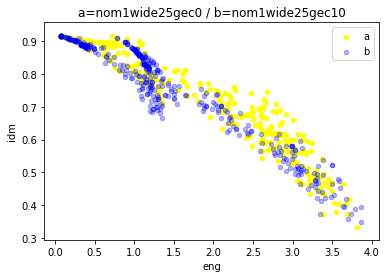
\includegraphics[width=1\linewidth,height=0.5\linewidth]{431.png}\vspace{2pt}
    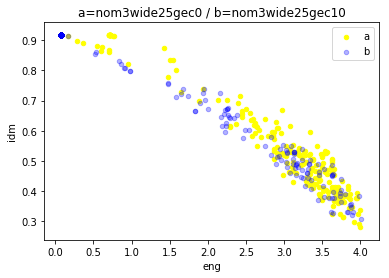
\includegraphics[width=1\linewidth,height=0.5\linewidth]{433.png}\vspace{2pt}
    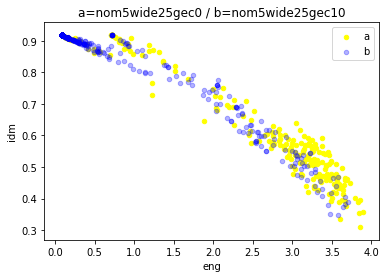
\includegraphics[width=1\linewidth,height=0.5\linewidth]{435.png}\vspace{2pt}
    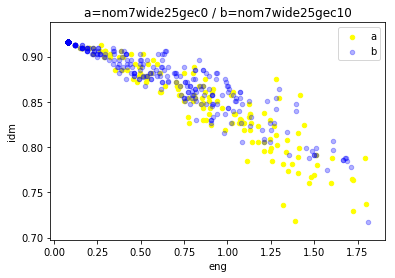
\includegraphics[width=1\linewidth,height=0.5\linewidth]{437.png}\vspace{2pt}
    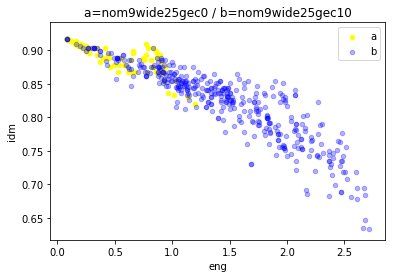
\includegraphics[width=1\linewidth,height=0.5\linewidth]{439.png}\vspace{2pt}
    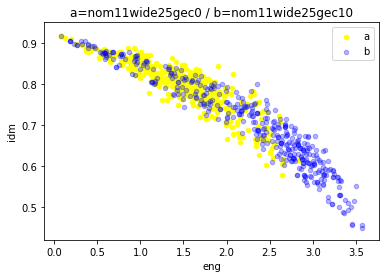
\includegraphics[width=1\linewidth,height=0.5\linewidth]{4311.png}\vspace{2pt}
    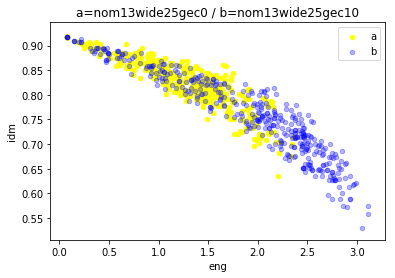
\includegraphics[width=1\linewidth,height=0.5\linewidth]{4313.png}
    \end{minipage}}
    \subfigure{
    \begin{minipage}[t]{0.45\linewidth}
    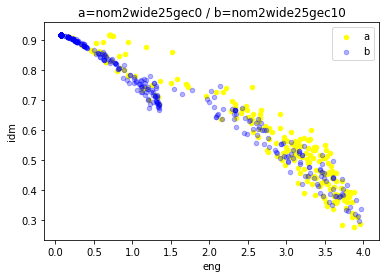
\includegraphics[width=1\linewidth,height=0.5\linewidth]{432.png}\vspace{2pt}
    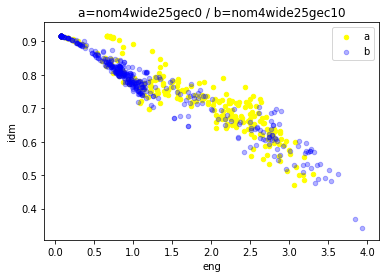
\includegraphics[width=1\linewidth,height=0.5\linewidth]{434.png}\vspace{2pt}
    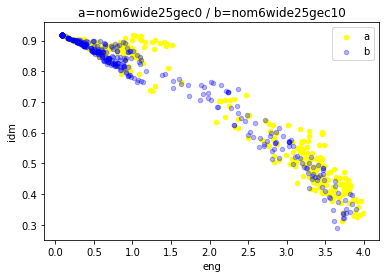
\includegraphics[width=1\linewidth,height=0.5\linewidth]{436.png}\vspace{2pt}
    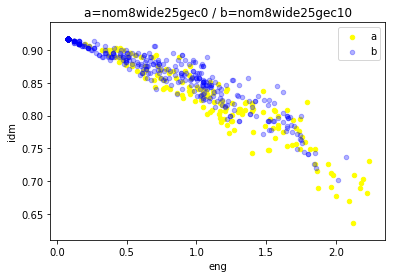
\includegraphics[width=1\linewidth,height=0.5\linewidth]{438.png}\vspace{2pt}
    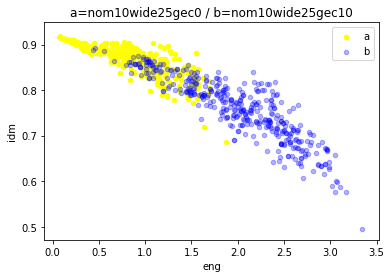
\includegraphics[width=1\linewidth,height=0.5\linewidth]{4310.png}\vspace{2pt}
    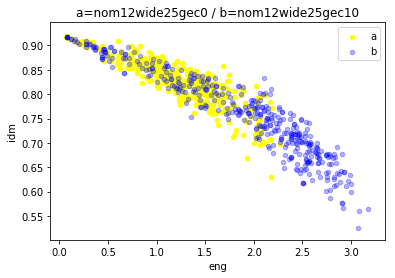
\includegraphics[width=1\linewidth,height=0.5\linewidth]{4312.png}\vspace{2pt}
    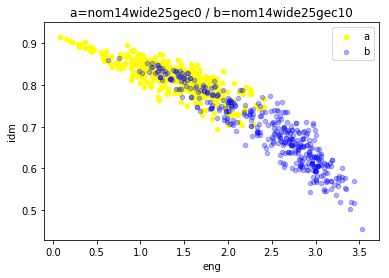
\includegraphics[width=1\linewidth,height=0.5\linewidth]{4314.png}
    \end{minipage}}
    \caption{不同波段纹理特征比较}
  \end{figure}

分析散点图可得:

1.低通道部分雷暴云类似线性聚集在一起,分析图像后发现,可见光通道和近红外通道在夜晚无法成像,
因此计算得出的纹理特征较为聚集。

2.观察5$\sim$10通道发现,雷暴云特征渐渐向图像右下方聚集,分析后得出,9、10通道介于中波红外与长波红外之间,
可以反映雷暴天气中的中高层水汽。

3.观察散点图可以发现中波红外到长波红外相比可见光和近红外更能反映雷暴信息。

实验证明了第三章提出的,在中长波红外和水汽通道能够较好反映出雷暴信息的结论。

\section{雷暴尺度及强度问题的实验验证}
\subsection{雷暴尺度问题}
图5.2中,nom1即表示1通道,共14个通道,wide25和wide50分别表示图像分辨率为25像素和50像素,
gec5表示雷暴强度大于5,将相同通道,相同雷暴强暴,相同纹理特征量(asm和con),
不同分辨率图像的纹理数据以散点图的形式表示,通过比较不同分辨率的图像,可以发现50像素分辨率相比25像素分辨率图像,
在各个通道都更为聚集。

\begin{figure}
    \centering
    \subfigure{
    \begin{minipage}[t]{0.45\linewidth}
    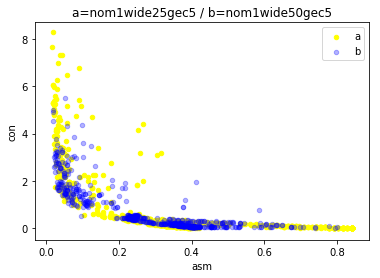
\includegraphics[width=1\linewidth,height=0.5\linewidth]{411.png}\vspace{2pt}
    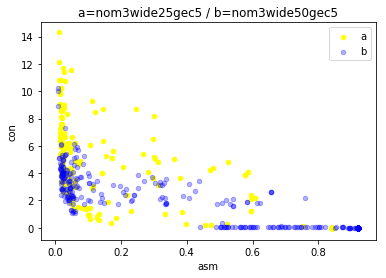
\includegraphics[width=1\linewidth,height=0.5\linewidth]{413.png}\vspace{2pt}
    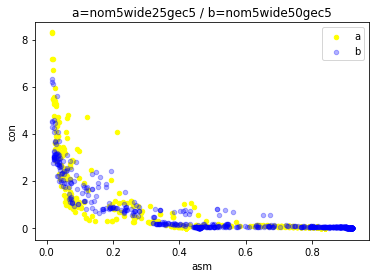
\includegraphics[width=1\linewidth,height=0.5\linewidth]{415.png}\vspace{2pt}
    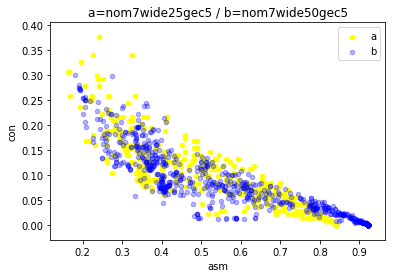
\includegraphics[width=1\linewidth,height=0.5\linewidth]{417.png}\vspace{2pt}
    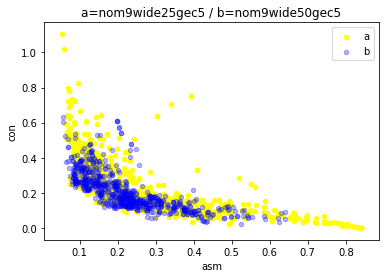
\includegraphics[width=1\linewidth,height=0.5\linewidth]{419.png}\vspace{2pt}
    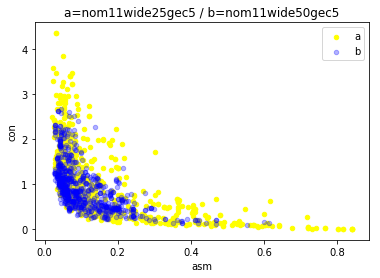
\includegraphics[width=1\linewidth,height=0.5\linewidth]{4111.png}\vspace{2pt}
    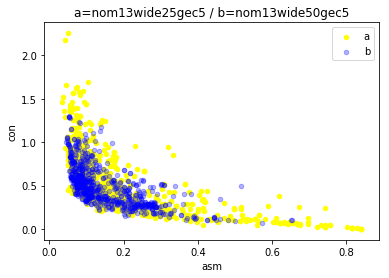
\includegraphics[width=1\linewidth,height=0.5\linewidth]{4113.png}
    \end{minipage}}
    \subfigure{
    \begin{minipage}[t]{0.45\linewidth}
    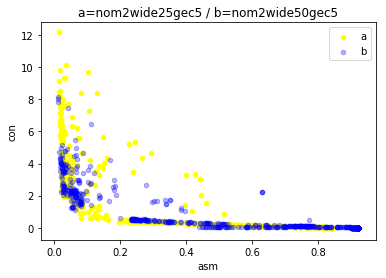
\includegraphics[width=1\linewidth,height=0.5\linewidth]{412.png}\vspace{2pt}
    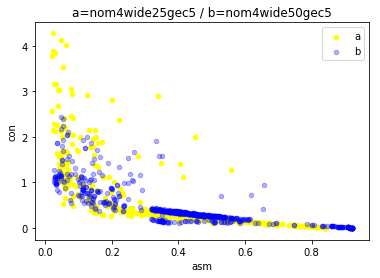
\includegraphics[width=1\linewidth,height=0.5\linewidth]{414.png}\vspace{2pt}
    \includegraphics[width=1\linewidth,height=0.5\linewidth]{416.png}\vspace{2pt}
    \includegraphics[width=1\linewidth,height=0.5\linewidth]{418.png}\vspace{2pt}
    \includegraphics[width=1\linewidth,height=0.5\linewidth]{4110.png}\vspace{2pt}
    \includegraphics[width=1\linewidth,height=0.5\linewidth]{4112.png}\vspace{2pt}
    \includegraphics[width=1\linewidth,height=0.5\linewidth]{4114.png}
    \end{minipage}}
    \caption{不同分辨率纹理特征比较}
  \end{figure}

\subsection{雷暴强度问题}
雷暴强度为闪电仪中获取到的闪电辐射值,下面将分析不同雷暴强度的图像,gec5表示雷暴强度介于5$\sim$10之间(标准化后数值),
gec10表示雷暴强度介于10$\sim$15之间,选取分辨率为25像素,纹理特征量取con和idm,各通道散点图如图5.3所示。

由各通道散点图可以看出,雷暴强度大于10的纹理特征相比雷暴强度介于5$\sim$10之间的纹理特征更为明显。


\begin{figure}
    \centering
    \subfigure{
    \begin{minipage}[t]{0.45\linewidth}
    \includegraphics[width=1\linewidth,height=0.5\linewidth]{421.png}\vspace{2pt}
    \includegraphics[width=1\linewidth,height=0.5\linewidth]{423.png}\vspace{2pt}
    \includegraphics[width=1\linewidth,height=0.5\linewidth]{425.png}\vspace{2pt}
    \includegraphics[width=1\linewidth,height=0.5\linewidth]{427.png}\vspace{2pt}
    \includegraphics[width=1\linewidth,height=0.5\linewidth]{429.png}\vspace{2pt}
    \includegraphics[width=1\linewidth,height=0.5\linewidth]{4211.png}\vspace{2pt}
    \includegraphics[width=1\linewidth,height=0.5\linewidth]{4213.png}
    \end{minipage}}
    \subfigure{
    \begin{minipage}[t]{0.45\linewidth}
    \includegraphics[width=1\linewidth,height=0.5\linewidth]{422.png}\vspace{2pt}
    \includegraphics[width=1\linewidth,height=0.5\linewidth]{424.png}\vspace{2pt}
    \includegraphics[width=1\linewidth,height=0.5\linewidth]{426.png}\vspace{2pt}
    \includegraphics[width=1\linewidth,height=0.5\linewidth]{428.png}\vspace{2pt}
    \includegraphics[width=1\linewidth,height=0.5\linewidth]{4210.png}\vspace{2pt}
    \includegraphics[width=1\linewidth,height=0.5\linewidth]{4212.png}\vspace{2pt}
    \includegraphics[width=1\linewidth,height=0.5\linewidth]{4214.png}
    \end{minipage}}
    \caption{不同雷暴强度纹理特征比较}
  \end{figure}

\section{纹理特征融合实验分析}
本文共计算了灰度共生矩阵的四种统计量,分别为asm,con,eng,idm,其中两两组合可以输出联合散点图,
共六种组合方式,选取第10通道,分辨率25,将非雷暴云和雷暴云进行比较,各通道散点图如图5.4所示。

由散点图可得,idm与eng联合,con与asm联合,asm与eng联合能够较为准确的反映雷暴云特征。

\begin{figure}
    \centering
    \subfigure{
    \begin{minipage}[t]{0.45\linewidth}
    \includegraphics[width=1\linewidth,height=0.5\linewidth]{441.png}\vspace{2pt}
    \includegraphics[width=1\linewidth,height=0.5\linewidth]{443.png}\vspace{2pt}
    \includegraphics[width=1\linewidth,height=0.5\linewidth]{445.png}
    \end{minipage}}
    \subfigure{
    \begin{minipage}[t]{0.45\linewidth}
    \includegraphics[width=1\linewidth,height=0.5\linewidth]{442.png}\vspace{2pt}
    \includegraphics[width=1\linewidth,height=0.5\linewidth]{444.png}\vspace{2pt}
    \includegraphics[width=1\linewidth,height=0.5\linewidth]{446.png}
    \end{minipage}}
    \caption{不同波段纹理特征比较}
  \end{figure}


\section{阈值提取}
针对以上分析,挑选出雷暴云与非雷暴云分类较为明显的散点图,如图5.5。

\begin{figure}
    \centering
    \subfigure{
    \begin{minipage}[t]{0.45\linewidth}
    \includegraphics[width=1\linewidth,height=0.5\linewidth]{451.png}\vspace{2pt}
    \includegraphics[width=1\linewidth,height=0.5\linewidth]{453.png}\vspace{2pt}
    \includegraphics[width=1\linewidth,height=0.5\linewidth]{455.png}
    \end{minipage}}
    \subfigure{
    \begin{minipage}[t]{0.45\linewidth}
    \includegraphics[width=1\linewidth,height=0.5\linewidth]{452.png}\vspace{2pt}
    \includegraphics[width=1\linewidth,height=0.5\linewidth]{454.png}\vspace{2pt}
    \includegraphics[width=1\linewidth,height=0.5\linewidth]{456.png}
    \end{minipage}}
    \caption{分类效果较好的散点图}
  \end{figure}

根据效果较好的散点图,提出了如下纹理特征阈值范围。
\begin{equation}
    0.78<eng(nom10)<3.50
\end{equation}
\begin{equation}
    0.09<con(nom10)<2.00 
\end{equation}
\begin{equation}
    0.50<idm(nom10)<0.90
\end{equation}
\begin{equation}
    0<asm(nom10)<0.40
\end{equation}

联合以上阈值范围,在一个包含400张雷暴云和400张非雷暴云的测试库中进行检测,
可以检测出370张雷暴图,119张非雷暴图,预警率为92.5$\%$,虚警率为29.75$\%$,
漏判率为24.34$\%$。
% !TeX root = ../main.tex

\chapter{总结与展望}
本文立足风云四号卫星影像数据,发挥气象卫星的优势,弥补地面设备雷电监测的缺陷,
讨论了卫星影像的图像特征以及针对风云四号云图雷暴提取的相关问题,
在建立图像样本库,计算图像特征数据的基础上,提出了雷暴云图的图像特征阈值范围。

基于地面设备的雷电监测,由于雷电的时空尺度较小等因素,目前难以实现实时对闪电的跟踪观测,
气象卫星则可以克服此缺陷,因此本文尝试从图像角度来提取雷暴云区的相关特征。
常用的图像特征主要有纹理特征,几何特征和频率特征等,而亮温差,有效对流位能和抬升指数
等指数和物理量也可以用来反映雷暴云区的特征。在图像特征基础上,本文又针对风云四号卫星,
从传感器波段、雷暴尺度强度和特征融合等问题进行了讨论分析。之后建立了样本库,
验证了理论分析结论的正确性,并通过数据分析提出了一套联合的图像特征阈值范围。
经测试库测试,预警率达到92.5$\%$,漏判率为24.34$\%$。

该方法的预警率达到理想精度,但漏判率偏高,表明研究中仍有不足之处,需要更加深入的研究。
首先是频率特征和几何特征,由于在实验过程中发现这两种特征在区分雷暴云和非雷暴云方面
效果不好,因此没有将此写入论文,也没有进行深入的研究,在以后的研究中将会从这两方面
特征入手,提高算法效率;其次是特征数据分析方面,没有进行数据的清洗,
选取的数据可视化方法也较为单一,因此分析得出的结论会有一定误差,下一步工作中
将考虑加入卷积神经网络的方法,提高算法的准确度。
% !TeX root = ../main.tex

\chapter{数学}

\section{数字和单位}

\begin{figure}
  \centering
  \subfigure{
  \begin{minipage}[t]{0.45\linewidth}
  \includegraphics[width=1\linewidth,height=0.7\linewidth]{439.png}\vspace{2pt}
  \includegraphics[width=1\linewidth,height=0.7\linewidth]{4311.png}\vspace{2pt}
  \includegraphics[width=1\linewidth,height=0.7\linewidth]{4313.png}
  \end{minipage}}
  \subfigure{
  \begin{minipage}[t]{0.45\linewidth}
  \includegraphics[width=1\linewidth,height=0.7\linewidth]{4310.png}\vspace{2pt}
  \includegraphics[width=1\linewidth,height=0.7\linewidth]{4312.png}\vspace{2pt}
  \includegraphics[width=1\linewidth,height=0.7\linewidth]{4314.png}
  \end{minipage}}
  \caption{不同波段纹理特征比较}
\end{figure}

\begin{figure}
  \centering
  \subfigure{
  \begin{minipage}[t]{0.30\linewidth}
  \includegraphics[width=1\linewidth,height=0.7\linewidth]{431.png}\vspace{2pt}
  \includegraphics[width=1\linewidth,height=0.7\linewidth]{434.png}\vspace{2pt}
  \includegraphics[width=1\linewidth,height=0.7\linewidth]{437.png}\vspace{2pt}
  \includegraphics[width=1\linewidth,height=0.7\linewidth]{4310.png}\vspace{2pt}
  \includegraphics[width=1\linewidth,height=0.7\linewidth]{4313.png}
  \end{minipage}}
  \subfigure{
  \begin{minipage}[t]{0.3\linewidth}
  \includegraphics[width=1\linewidth,height=0.7\linewidth]{432.png}\vspace{2pt}
  \includegraphics[width=1\linewidth,height=0.7\linewidth]{435.png}\vspace{2pt}
  \includegraphics[width=1\linewidth,height=0.7\linewidth]{438.png}\vspace{2pt}
  \includegraphics[width=1\linewidth,height=0.7\linewidth]{4311.png}\vspace{2pt}
  \includegraphics[width=1\linewidth,height=0.7\linewidth]{4314.png}
  \end{minipage}}
  \subfigure{
  \begin{minipage}[t]{0.3\linewidth}
  \includegraphics[width=1\linewidth,height=0.7\linewidth]{433.png}\vspace{2pt}
  \includegraphics[width=1\linewidth,height=0.7\linewidth]{436.png}\vspace{2pt}
  \includegraphics[width=1\linewidth,height=0.7\linewidth]{439.png}\vspace{2pt}
  \includegraphics[width=1\linewidth,height=0.7\linewidth]{4312.png}
  \end{minipage}}
  \caption{不同波段纹理特征比较}
\end{figure}

\begin{figure}
  \centering
  \subfigure{
  \begin{minipage}[t]{0.46\linewidth}
  \includegraphics[width=1\linewidth,height=0.5\linewidth]{纹理特征分析方法1.png}\vspace{4pt}
  \includegraphics[width=1\linewidth,height=0.5\linewidth]{纹理特征分析方法1.png}
  \end{minipage}}
  \subfigure{
  \begin{minipage}[t]{0.46\linewidth}
  \includegraphics[width=1\linewidth]{纹理特征分析方法1.png}\vspace{4pt}
  \includegraphics[width=1\linewidth]{纹理特征分析方法1.png}
  \end{minipage}}
  \caption{description of figure}
  \end{figure}



宏包 \pkg{siunitx} 提供了更好的数字和单位支持:
\begin{itemize}
  \item \num{12345.67890}
  \item \num{1+-2i}
  \item \num{.3e45}
  \item \num{1.654 x 2.34 x 3.430}
  \item \si{kg.m.s^{-1}}
  \item \si{\micro\meter} $\si{\micro\meter}$
  \item \si{\ohm} $\si{\ohm}$
  \item \numlist{10;20}
  \item \numlist{10;20;30}
  \item \SIlist{0.13;0.67;0.80}{\milli\metre}
  \item \numrange{10}{20}
  \item \SIrange{10}{20}{\degreeCelsius}
\end{itemize}



\section{数学符号和公式}

\LaTeX{} 默认按照美国的习惯排版数学公式和符号,
但是《撰写手册》要求数学符号依据《GB 3102.11--1993》执行,
与 \LaTeX{} 的习惯有所差异。
本模板基于 \pkg{unicode-math} 配置数学符号,以遵循国标的规定。

注意,\pkg{unicode-math} 宏包与 \pkg{amsfonts}, \pkg{amssymb}, \pkg{bm},
\pkg{mathrsfs}, \pkg{upgreek} 等宏包\emph{不}兼容。
本模板作了处理,用户可以直接使用这些宏包的命令,如 \cs{bm}, \cs{mathscr},
\cs{upGamma}。

本模板中数学符号的用法与 \LaTeX{} 传统有些区别:
\begin{itemize}
  \item 数学常数和特殊函数使用正体,
    如圆周率 $\symup{\pi}$、$\symup{\Gamma}$ 函数。
    应使用 \pkg{unicode-math} 宏包提供的 \cs{symup} 命令转为正体,
    如 \verb|\symup{\pi}|。
  \item 向量和矩阵粗斜体,应使用 \cs{symbf} 命令,
    如 \verb|\symbf{u}|、\verb|\symbf{A}|。
  \item 有限增量符号 $\increment$ (U+2206)应使用 \cs{increment} 命令。
  \item 微分符号 $\dif$ 使用正体,本模板提供了 \cs{dif} 命令。
\end{itemize}

除此之外,模板还提供了一些命令方便使用:
\begin{itemize}
  \item 常数 $\upe$:\verb|\upe|
  \item 负数单位 $\upi$:\verb|\upi|
  \item 圆周率 $\uppi$:\verb|\uppi|
  \item $\argmax$:\verb|\argmax|
  \item $\argmin$:\verb|\argmin|
\end{itemize}

关于数学符号更多的用法,参见 \pkg{unicode-math} 宏包的使用说明和符号列表
\pkg{unimath-symbols}。

在编辑数学公式时,最好避免直接使用字体命令,
而应该定义一些语义命令取代字体命令,
这样输入更简单,也让 \LaTeX{} 代码更有可读性,
而且还方便根据需要统一修改改格式,比如:
\begin{itemize}
  \item 向量 $\vec{x}$:\verb|\renewcommand\vec{\symbf}|
  \item 矩阵 $\mat{A}$:\verb|\newcommand\mat{\symbf}|
  \item 张量 $\ts{T}$: \verb|\newcommand\ts{\symbfsf}|
\end{itemize}

更多的例子:
\begin{equation}
  \upe^{\upi\uppi} + 1 = 0
\end{equation}
\begin{equation}
  \frac{\dif^2 u}{\dif t^2} = \int f(x) \dif x
\end{equation}
\begin{equation}
  \argmin_x f(x)
\end{equation}
\begin{equation}
  \mat{A} \vec{x} = \lambda \vec{x}
\end{equation}



\section{定理和证明}

示例文件中使用 \pkg{amsthm} 宏包配置了定理、引理和证明等环境。
用户也可以使用  \pkg{ntheorem} 宏包。

\begin{definition}
  If the integral of function $f$ is measurable and non-negative, we define
  its (extended) \textbf{Lebesgue integral} by
  \begin{equation}
    \int f = \sup_g \int g,
  \end{equation}
  where the supremum is taken over all measurable functions $g$ such that
  $0 \le g \le f$, and where $g$ is bounded and supported on a set of
  finite measure.
\end{definition}

\begin{assumption}
The communication graph is strongly connected.
\end{assumption}

\begin{example}
  Simple examples of functions on $\real^d$ that are integrable
  (or non-integrable) are given by
  \begin{equation}
    f_a(x) =
    \begin{cases}
      |x|^{-a} & \text{if } |x| \le 1, \\
      0        & \text{if } x > 1.
    \end{cases}
  \end{equation}
  \begin{equation}
    F_a(x) = \frac{1}{1 + |x|^a}, \qquad \text{all } x \in \real^d.
  \end{equation}
  Then $f_a$ is integrable exactly when $a < d$, while $F_a$ is integrable
  exactly when $a > d$.
\end{example}

\begin{lemma}[Fatou]
  Suppose $\{f_n\}$ is a sequence of measurable functions with $f_n \geq 0$.
  If $\lim_{n \to \infty} f_n(x) = f(x)$ for a.e. $x$, then
  \begin{equation}
    \int f \le \liminf_{n \to \infty} \int f_n.
  \end{equation}
\end{lemma}

\begin{remark}
  We do not exclude the cases $\int f = \infty$,
  or $\liminf_{n \to \infty} f_n = \infty$.
\end{remark}

\begin{corollary}
  Suppose $f$ is a non-negative measurable function, and $\{f_n\}$ a sequence
  of non-negative measurable functions with
  $f_n(x) \le f(x)$ and $f_n(x) \to f(x)$ for almost every $x$. Then
  \begin{equation}
    \lim_{n \to \infty} \int f_n = \int f.
  \end{equation}
\end{corollary}

\begin{proposition}
  Suppose $f$ is integrable on $\real^d$. Then for every $\epsilon > 0$:
  \begin{enumerate}
    \renewcommand{\theenumi}{\roman{enumi}}
    \item There exists a set of finite measure $B$ (a ball, for example) such
      that
      \begin{equation}
        \int_{B^c} |f| < \epsilon.
      \end{equation}
    \item There is a $\delta > 0$ such that
      \begin{equation}
        \int_E |f| < \epsilon \qquad \text{whenever } m(E) < \delta.
      \end{equation}
  \end{enumerate}
\end{proposition}

\begin{theorem}
  Suppose $\{f_n\}$ is a sequence of measurable functions such that
  $f_n(x) \to f(x)$ a.e. $x$, as $n$ tends to infinity.
  If $|f_n(x)| \le g(x)$, where $g$ is integrable, then
  \begin{equation}
    \int |f_n - f| \to 0 \qquad \text{as } n \to \infty,
  \end{equation}
  and consequently
  \begin{equation}
    \int f_n \to \int f \qquad \text{as } n \to \infty.
  \end{equation}
\end{theorem}

\begin{proof}
  Trivial.
\end{proof}

\newtheorem*{axiomofchoice}{Axiom of choice}
\begin{axiomofchoice}
  Suppose $E$ is a set and ${E_\alpha}$ is a collection of
  non-empty subsets of $E$. Then there is a function $\alpha
  \mapsto x_\alpha$ (a ``choice function'') such that
  \begin{equation}
    x_\alpha \in E_\alpha,\qquad \text{for all }\alpha.
  \end{equation}
\end{axiomofchoice}

\newtheorem{observation}{Observation}
\begin{observation}
  Suppose a partially ordered set $P$ has the property
  that every chain has an upper bound in $P$. Then the
  set $P$ contains at least one maximal element.
\end{observation}
\begin{proof}[A concise proof]
  Obvious.
\end{proof}


\section{三线表}

三线表是《撰写手册》推荐使用的格式,如表~\ref{tab:exampletable}。
\begin{table}[htb]
  \centering\small
  \caption{表号和表题在表的正上方}
  \label{tab:exampletable}
  \begin{tabular}{cl}
    \toprule
    类型   & 描述                                       \\
    \midrule
    挂线表 & 挂线表也称系统表、组织表,用于表现系统结构 \\
    无线表 & 无线表一般用于设备配置单、技术参数列表等   \\
    卡线表 & 卡线表有完全表,不完全表和三线表三种       \\
    \bottomrule
  \end{tabular}
  \note{注:表注分两种,第一种是对全表的注释,用不加阿拉伯数字排在表的下边,
    前面加“注:”;第二种是和表内的某处文字或数字相呼应的注,
    在表里面用带圈的阿拉伯数字在右上角标出,然后在表下面用同样的圈码注出来}
\end{table}

编制表格应简单明了,表达一致,明晰易懂,表文呼应、内容一致。
排版时表格字号略小,或变换字体,尽量不分页,尽量不跨节。
表格太大需要转页是,需要在续表上方注明“续表”,表头页应重复排出。



\section{插图}

有的同学可能听说“\LaTeX{} 只能使用 eps 格式的图片”,甚至把 jpg 格式转为 eps。
事实上,这种做法已经过时。
而且每次编译时都要要调用外部工具解析 eps,导致降低编译速度。
所以我们推荐矢量图直接使用 pdf 格式,位图使用 jpeg 或 png 格式。
\begin{figure}[htb]
  \centering
  \includegraphics[width=0.3\textwidth]{ustc_logo_fig.pdf}
  \caption{图号、图题置于图的下方}
  \label{fig:logo}
  \note{注:图注的内容不宜放到图题中。}
\end{figure}

关于图片的并排,推荐使用较新的 \pkg{subcaption} 宏包,
不建议使用 \pkg{subfigure} 或 \pkg{subfig} 等宏包。



\section{算法环境}

模板中使用 \pkg{algorithm2e} 宏包实现算法环境。关于该宏包的具体用法,
请阅读宏包的官方文档。

\begin{algorithm}[htb]
  \small
  \SetAlgoLined
  \KwData{this text}
  \KwResult{how to write algorithm with \LaTeX2e }

  initialization\;
  \While{not at end of this document}{
    read current\;
    \eIf{understand}{
      go to next section\;
      current section becomes this one\;
    }{
      go back to the beginning of current section\;
    }
  }
  \caption{算法示例1}
  \label{algo:algorithm1}
\end{algorithm}

注意,我们可以在论文中插入算法,但是插入大段的代码是愚蠢的。
然而这并不妨碍有的同学选择这么做,对于这些同学,建议用 \pkg{listings} 宏包。

\mainmatter
\chapter{Citations}

\citet{knuth86a}
\citet[42]{knuth86a}

\citep{knuth86a}
\citep[42]{knuth86a}
\citep[see][]{knuth86a}
\citep[see][42]{knuth86a}

\citet*{tlc2}
\citep*{tlc2}

\citet{knuth86a,tlc2}
\citep{knuth86a,tlc2}
\citep{knuth86a,knuth84}
\citep{knuth86a,knuth86b}

\citet{knuth86b,knuth86a,knuth84}
\citep{knuth86b,knuth86a,knuth84}

\cite{slg,cgw,kqy,dwx,jxz,wjk,syw}

\bibliography{refs}


\appendix
%% !TeX root = ../main.tex

\chapter{补充材料}


补充内容。


\backmatter
% !TeX root = ../main.tex

\begin{acknowledgements}

    时光飞逝,大学四年时光转眼间已经临近尾声。
    首先,要感谢学校搭建了优质的学习平台,提供了不错的学习环境,
    让我接触到无数优秀的老师和同学,在与老师和同学的相处过程中不断提高自己,
    丰富多彩的校园生活让我在南航度过了四年快乐的时光,我始终为自己是一名南航人而感到自豪和骄傲。
    其次,要感谢王博老师和盛庆红老师,正是本科阶段你们的悉心引导,让我找到了心中真正喜欢的领域,
    确定了未来的发展方向,在论文撰写期间的监督指导,为我毕业论文的顺利完成提供了莫大的帮助;
    再次,要感谢我的父母,取得进展的时候和你们一起分享成功的喜悦,遇到难题的时候也总是给我支持鼓励。

    最后,还要感谢课题组学长学姐,谢谢你们帮我寻找解决问题的思路;
    感谢足球队的兄弟,和你们一起踢球是我大学最美好的回忆;
    感谢身边的同学朋友,有你们的陪伴让我充满了力量。愿未来,大家一切都好!

\end{acknowledgements}

%% !TeX root = ../main.tex

\begin{publications}

\section*{已发表论文}

\begin{enumerate}
\item A A A A A A A A A
\item A A A A A A A A A
\item A A A A A A A A A
\end{enumerate}

\section*{待发表论文}

\begin{enumerate}
\item A A A A A A A A A
\item A A A A A A A A A
\item A A A A A A A A A
\end{enumerate}

\section*{研究报告}
\begin{enumerate}
\item A A A A A A A A A
\item A A A A A A A A A
\item A A A A A A A A A
\end{enumerate}

\end{publications}


\end{document}
